%==============================================================
%  Metadata-Augmented Recursive Decomposition (MARD)
%  Manuscript A  --  IEEE conference format
%
%  Upload to Overleaf as a new project; main file = this file.
%  Compiler: pdfLaTeX.  IEEEtran.cls is available on Overleaf by
%  default, so no .cls upload is required.
%
%  MERGED 27 Aug 2026: team layout (author block, section
%  numbering, Fig. 1, inline bibliography) + the groundedness /
%  methodology material from the working draft.
%
%  TWO PLACEHOLDER CONVENTIONS, both greppable:
%    % >>> PENDING   prose that still needs writing
%    \RESULT         a table cell with no measured number yet
%                    (prints a red marker, so an unfilled cell can
%                    never be mistaken for an em-dash or a zero)
%  Before the final build, delete the three macro definitions
%  below: the document then FAILS to compile if any \TODO,
%  \VERIFY or \RESULT survived. That is deliberate.
%==============================================================
\documentclass[conference]{IEEEtran}
\IEEEoverridecommandlockouts
\usepackage{cite}
\usepackage{amsmath,amssymb,amsfonts}
\usepackage{algorithm}
\usepackage{algorithmic}
\usepackage{graphicx}
\usepackage{textcomp}
\usepackage{xcolor}
\usepackage{booktabs}
\usepackage{array}
\usepackage{siunitx}
\usepackage{url}
\usepackage{tikz}
\usetikzlibrary{arrows.meta,positioning,fit,backgrounds}

% --- Draft markers. DELETE these three lines for the final build. ---------
\newcommand{\TODO}[1]{\textcolor{red}{\textbf{[TODO: #1]}}}
\newcommand{\VERIFY}[1]{\textcolor{orange}{\textbf{[VERIFY: #1]}}}
\newcommand{\RESULT}{\textcolor{red}{\textbf{--}}}

% --- Figure 1 palette (print-safe; distinguishable in greyscale) ---------
\definecolor{mardblue}{HTML}{1F5FA9}   % Tier 1 -- Scout
\definecolor{mardbluebg}{HTML}{EAF2FB}
\definecolor{mardorange}{HTML}{C05621} % Tier 2 -- Builders
\definecolor{mardorangebg}{HTML}{FDF0E6}
\definecolor{mardink}{HTML}{16202B}    % Master Plan
\definecolor{mardgrey}{HTML}{6B7785}   % Document / output

% --- Section numbering: arabic sections, dotted subsections (1, 1.1, 1.1.1) ---
% IEEEtran keeps TWO sets of labels: \thesection... drives \ref and the ToC,
% while \thesection...dis drives what is printed in the heading itself. Both
% must be overridden, or headings keep showing "A." "B." "C.".
\renewcommand{\thesection}{\arabic{section}}
\renewcommand{\thesubsection}{\thesection.\arabic{subsection}}
\renewcommand{\thesubsubsection}{\thesubsection.\arabic{subsubsection}}
\renewcommand{\theparagraph}{\thesubsubsection.\arabic{paragraph}}
\renewcommand{\thesectiondis}{\arabic{section}.}
\renewcommand{\thesubsectiondis}{\arabic{section}.\arabic{subsection}.}
\renewcommand{\thesubsubsectiondis}{%
  \arabic{section}.\arabic{subsection}.\arabic{subsubsection}.}
\renewcommand{\theparagraphdis}{%
  \arabic{section}.\arabic{subsection}.\arabic{subsubsection}.\arabic{paragraph}.}

\sisetup{group-separator={,}, detect-weight=true}
% Column type for right-aligned numeric columns of fixed width
\newcolumntype{R}[1]{>{\raggedleft\arraybackslash}p{#1}}

\def\BibTeX{{\rm B\kern-.05em{\sc i\kern-.025em b}\kern-.08em
    T\kern-.1667em\lower.7ex\hbox{E}\kern-.125emX}}

\begin{document}
\title{Metadata-Augmented Recursive Decomposition for\\
Cost-Efficient Comprehension of Unbounded Documents}

\author{%
\begin{tabular}{@{}*{5}{>{\centering\arraybackslash}p{0.19\textwidth}}@{}}
Parth Sangani\textsuperscript{1,\,a,\,b,\,*} &
Arav Sharma\textsuperscript{2,\,a,\,b} &
Anugrah Shetty\textsuperscript{3,\,a,\,b} &
Tanish Sharma\textsuperscript{4,\,a,\,b} &
Soni Sweta\textsuperscript{5,\,a,\,b}
\end{tabular}\\[4pt]
{\footnotesize\textsuperscript{a}Department of Computer Engineering}\\[1pt]
{\footnotesize\textsuperscript{b}Mukesh Patel School of Technology Management \& Engineering, SVKM's Narsee Monjee}\\[1pt]
{\footnotesize Institute of Management Studies (NMIMS) Deemed-to-University, Mumbai-400056, India}\\[4pt]
{\footnotesize\textsuperscript{1}\texttt{sanganiparth22@gmail.com}}\\[1pt]
{\footnotesize\textsuperscript{2}\texttt{arav.sharma0405@gmail.com}}\\[1pt]
{\footnotesize\textsuperscript{3}\texttt{anuadz2358@gmail.com}}\\[1pt]
{\footnotesize\textsuperscript{4}\texttt{tanishsharma619@gmail.com}}\\[1pt]
{\footnotesize\textsuperscript{5}\texttt{soni.sweta16@gmail.com}}\\[2pt]
{\footnotesize Corresponding Author\textsuperscript{*}}%
}
\maketitle

\begin{abstract}
Recursive Language Models (RLMs) process inputs far beyond a model's
native context window by holding the document in a REPL environment and
letting a root model explore it programmatically, delegating reading to
sub-model calls. We observe that this exploration is structurally blind:
each recursive call receives a raw text slice with no view of the
document's organisation, no record of what sibling calls have already
established, and no statement of why it was invoked. On documents whose
structure is exploitable---textbooks, manuals, standards---this discards
precisely the information that makes the document navigable. We propose
Metadata-Augmented Recursive Decomposition (MARD), an inference-time
extension that threads a metadata envelope through every recursive call.
The envelope carries a structural skeleton derived from the document's own
text, findings accumulated from prior calls, and a parent-issued directive,
and it grows as exploration proceeds. Exploration thereby becomes an act of
confirming a hypothesis rather than of discovering blindly. We instantiate
MARD on dependency-ordered study-material generation over textbook-scale
documents, where a frontier ``Scout'' reads a small fraction of the document
to emit a typed Master Plan and a fleet of cheap ``Swarm'' builders generate
material that is joined in dependency order rather than book order. We
evaluate MARD against vanilla RLM under matched models, matched recursion
depth and identical structural controls, measuring output quality and tokens
consumed independently, with three repeated runs per condition and a
flat-context negative control. We additionally instrument the
\emph{groundedness} of generated content, after observing the baseline
silently produce explanations without consulting the source document while
reporting success.
On explanation coverage the two arms are indistinguishable---MARD $0.621$
against the baseline's $0.551$, over ranges that overlap---and we report that
as a null. The contribution is elsewhere. MARD consumes $15.8\times$ fewer
input tokens, and it is stable where the baseline is not: across three
identical repeats the baseline's coverage ranges from $0.315$ to $0.765$ and
its output organisation from $75$ to $190$ sections, while MARD's range
$0.584$--$0.650$ and $83$--$84$ concepts, each carrying a source span that
resolves against the document; the baseline emits no resolvable citation in
any repeat. Ablating the envelope by channel isolates the mechanism: removing
the accumulated findings collapses cross-chapter dependency linkage from
$0.917$ to $0.014$, while removing the structural skeleton---the most
expensive component of the frontier tier's input---changes nothing we can
measure. On a structure-ablated document MARD declines to run at zero cost,
whereas the baseline produces confident study guides that acknowledge no
disorder. We report two limitations that bound these claims: MARD's builders
never receive the cited prose, so its explanations are attributable but not
text-grounded, and we did not reproduce a published baseline result
first-hand.
\end{abstract}

\begin{IEEEkeywords}
long-context language models, recursive inference, document structure,
prerequisite ordering, inference-time methods, cost-efficient inference
\end{IEEEkeywords}

\section{Introduction}
\label{sec:intro}
The dominant approach to reasoning over documents that exceed a language
model's context window is to reduce the document: chunk and retrieve,
compress the prompt, or compact the conversation. Each discards information
and each does so before the model has had a chance to decide what matters.

Recursive Language Models \cite{zhang2025rlm} invert this. The document is
never placed in the prompt at all. It is bound to a variable inside a Python
REPL, and the root model receives only metadata about it---its type, its
length. The root then writes code to explore it: slicing, regular
expressions, loops. Inside that REPL it may call \texttt{llm\_query}, handing
an extracted slice to a sub-model that reads it and returns an answer. The
root is an orchestrator that decides what to read and delegates the reading.
Because the root sees only truncated program output, its own context grows
slowly, and inputs of several million tokens become tractable against a
context window two orders of magnitude smaller.

\subsection{The defect: recursion without orientation}
\label{sec:gap}
We observe a specific deficiency in this design. Every sub-call is given a
raw slice of text and nothing else. It does not know which document the slice
comes from, where in that document it sits, what other sub-calls have already
established, or why it in particular was invoked. It is, in effect, a reader
handed three photocopied pages with no cover and no page numbers.

Two costs follow. First, orientation is re-derived on every call rather than
established once and reused. Second, sub-calls cannot build on one another:
a finding established in Chapter~3 is unavailable to the call that reads
Chapter~9, even though the document itself may explicitly connect them. On a
flat context---a shuffled transcript, a log file---neither cost is avoidable,
because there is no structure to be oriented against. But on a document with
exploitable structure, the information being discarded is exactly the
information the author supplied to make the text navigable: a table of
contents, numbered sections, and in-text cross-references of the form ``as we
saw in Chapter~3.''

\subsection{Contribution}
We introduce a \emph{metadata envelope}: a compact, growing structure carried
into every recursive call, comprising (i)~a structural skeleton of the
document, (ii)~findings accumulated across prior calls, and (iii)~a directive
issued by the calling context stating what this call is for. Our claim,
stated in the form we commit to before reporting any measurement:

\begin{quote}
MARD's growing metadata envelope makes recursive document exploration
structure-aware---improving output quality and/or reducing tokens consumed
relative to vanilla RLM on documents with exploitable structure, while
degrading gracefully to vanilla-RLM behaviour on documents without it.
\end{quote}

Three properties of this sentence are deliberate. It credits the envelope,
not recursion, because recursion is the base paper's. It is a disjunction
over quality and tokens, because we do not know in advance which axis the
effect appears on and measure both independently. And the
graceful-degeneration clause is a prediction stated in advance, not a failure
mode discovered afterwards; it is an objective of this work rather than a
caveat on it.

A second property emerged from measurement rather than design, and we report
it as a finding rather than folding it into the claim above. Because MARD's
plan is a \emph{typed contract} validated at the tier boundary, a builder
receives its source span by construction rather than by a model matching text
to a concept at generation time. We observed the vanilla baseline silently
generate content without consulting the document at all, while reporting
success (Section~\ref{sec:grounding}). The envelope's structural apparatus
makes that failure mode loud rather than silent, which is a claim about
\emph{faithfulness and auditability} distinct from output quality.

\subsection{What is not claimed}
It is important to say this before a reader infers otherwise. The base
paper's RLM already pairs a frontier root model with cheaper sub-model calls,
and already recurses. Neither is our contribution. The base library that
accompanies it already carries rich per-call metadata and even ships an
example demonstrating metadata captured at every depth of the recursion tree.
Section~\ref{sec:baselib} draws the line precisely: that metadata flows
upward and is observational, whereas MARD's envelope flows downward and is
operative. Same word, opposite direction, and only one of the two changes
what the model does.

We also make no claim to beat the state of the art on long-context
benchmarks. Isolating MARD's contribution means comparing against vanilla
RLM; the base paper's own results report a higher overall high-water mark
from a different system, and that remains the standing bar
\cite{zhang2025rlm}.

\subsection{Demonstrating application}
We instantiate MARD on the generation of dependency-ordered study material
from textbook-scale documents. This application is chosen because it makes
the envelope's contribution measurable rather than anecdotal: a textbook
declares its own prerequisite relations through in-text cross-references, so
a generated ordering can be scored against ground truth extracted
programmatically from the document itself, with no expert annotation and
therefore no human-subjects component.

The application also traces a specific engineering path, and naming it makes
the design constraints legible. A structured view of a document can be
obtained directly, by handing the source to a long-context model and rendering
the structure it emits; this is the shape of the tools in
Fig.~\ref{fig:trees}(a) and (b). That approach is bounded by the context
window, which a textbook exceeds. Recursive Language Models remove the bound
by never placing the document in a prompt---but our measurements show that
what they return in its place is unstable. Across three repeats of an
identical configuration the baseline's output organisation ranged from
\num{75} to \num{190} sections (Section~\ref{sec:variance}), and given a
document whose structure had been destroyed it produced three confident study
guides that named the intact book's opening section and acknowledged nothing
(Section~\ref{sec:negcontrol}). A structure extracted once, by hand, can be
inspected before it is trusted; a structure extracted on every run, varying
this much, cannot.

MARD is the attempt to keep the recursion and recover the stability. What it
produces is not the study text itself but a \emph{concept graph}: concepts
carrying verified source sections and page ranges, joined by prerequisite
edges. That artefact is the object we intend to be rendered and navigated---an
ordering over a book that reflects what must be understood before what,
rather than the order in which the pages happen to be bound.

We are explicit that this manuscript does not evaluate that end. No learner
used the artefact, no comparison against linear reading was run, and no claim
about learning outcomes is made or implied anywhere in this paper. What is
evaluated is whether the artefact can be produced reliably, cheaply and with
checkable provenance, which is the precondition for asking the learning
question at all.

\section{Literature Review}
\label{sec:related}

\subsection{Recursive and long-context inference}
Our work extends RLM \cite{zhang2025rlm} directly. A recent alternative
framework, SRLM \cite{alizadeh2026srlm}, reports up to \num{22}\% over RLM
under a matched time budget and argues that recursion may not be the primary
driver of RLM's advantage, observing that within-window
recursion sometimes degrades performance. We take no position on that
dispute, and our design does not require one: the envelope reduces
orientation cost, which is a claim about what each call is \emph{given}
rather than about what makes recursion work. The critique does, however,
shape our methodology. If the objection to a reported improvement is that it
may be sampling noise or prompt luck, the defence is not more documents but
variance across repeated runs, a negative control, and a boundary condition
stated in advance. Section~\ref{sec:setup} adopts all three.

Positional-degradation results \cite{liu2024lost} motivate the broader family
of context-reduction approaches, of which prompt compression
\cite{jiang2023llmlingua,pan2024llmlingua2,li2023compressing} and its recent
survey \cite{li2025survey} are representative. These are complementary rather
than competing: they reduce what a call must read, whereas MARD changes what
a call knows about what it reads.

\subsection{Hierarchical decomposition of long documents}
Hierarchical merging for summarisation \cite{ou2025hierarchical} and
multi-agent narrative summarisation \cite{kim2025nexussum} decompose long
inputs into a tree and combine partial results upward. The structural
difference from MARD is the direction of information flow: in merging
schemes, context is assembled on the way up. In MARD, accumulated context is
injected on the way down, before each unit of work executes.

\subsection{Tiered and cost-aware inference}
Routing and cascading approaches \cite{ong2024routellm,moslem2026routing} and
hint-based delegation \cite{dong2026hints} allocate a frontier model
selectively to control cost. MARD's Scout/Swarm split is an instance of the
same economics, and we claim no novelty for it. What is ours is that the
cheap tier receives a typed plan directive rather than an undifferentiated
slice---an ablation we isolate directly (Section~\ref{sec:ablation}).

\subsection{Prerequisite structure and educational applications}
Concept prerequisite extraction has an established literature
\cite{li2021prereq,sun2024learningpath,prereqsurvey2025}, as do LLM agents in
education \cite{wu2025agents,tufino2025notebooklm}. The application context
these serve---adaptive and personalised e-learning, and the educational data
mining that supports it---is surveyed in \cite{sweta2021edm}. We differ in the
source of supervision: rather than learning prerequisite relations from labelled
corpora, we treat each edge our system emits as a falsifiable prediction
against the document's own declared cross-references.

\subsection{Positioning against shipped systems}
Two acknowledgements, which we state rather than let a reader supply.
Ingestion capacity is not the gap---deployed products already accept large
document collections---and at least one shipped product now generates
sequenced study plans from uploaded course material. The line we draw is on
the \emph{source} of the sequencing: deployed systems that sequence do so
diagnostically, ordering by what a learner has answered incorrectly, whereas
our ordering is document-derived, extracted without supervision and scored
against the text's own cross-references. We deliberately do not use any
closed product as a quantitative baseline: their architectures are
unpublished, they expose no token accounting, and they change without notice,
so no such comparison would reproduce.
No peer-reviewed source establishes what any particular shipped product's
mind-map view does or does not encode, so we treat this as a qualitative
observation supported by first-hand inspection rather than as a citable claim.
Fig.~\ref{fig:trees} places three renderings of the same source document side
by side. The distinction it is intended to make visible is not depth or
resolution but \emph{edge semantics}: in panels (a) and (b) an edge means
\emph{is contained in}, and in panel (c) an edge means \emph{must precede}.
Panels (a) and (b) are first-hand screenshots taken on 27~August~2026. They
are reproducible only in the sense that the procedure is stated: both products
are closed and change without notice, so a reader running the same steps later
may see a different rendering. We state the capture date for that reason and
make no claim about either product's behaviour beyond that date.

\begin{figure*}[!t]
\centering
\begin{minipage}[t]{0.47\textwidth}
  \centering
  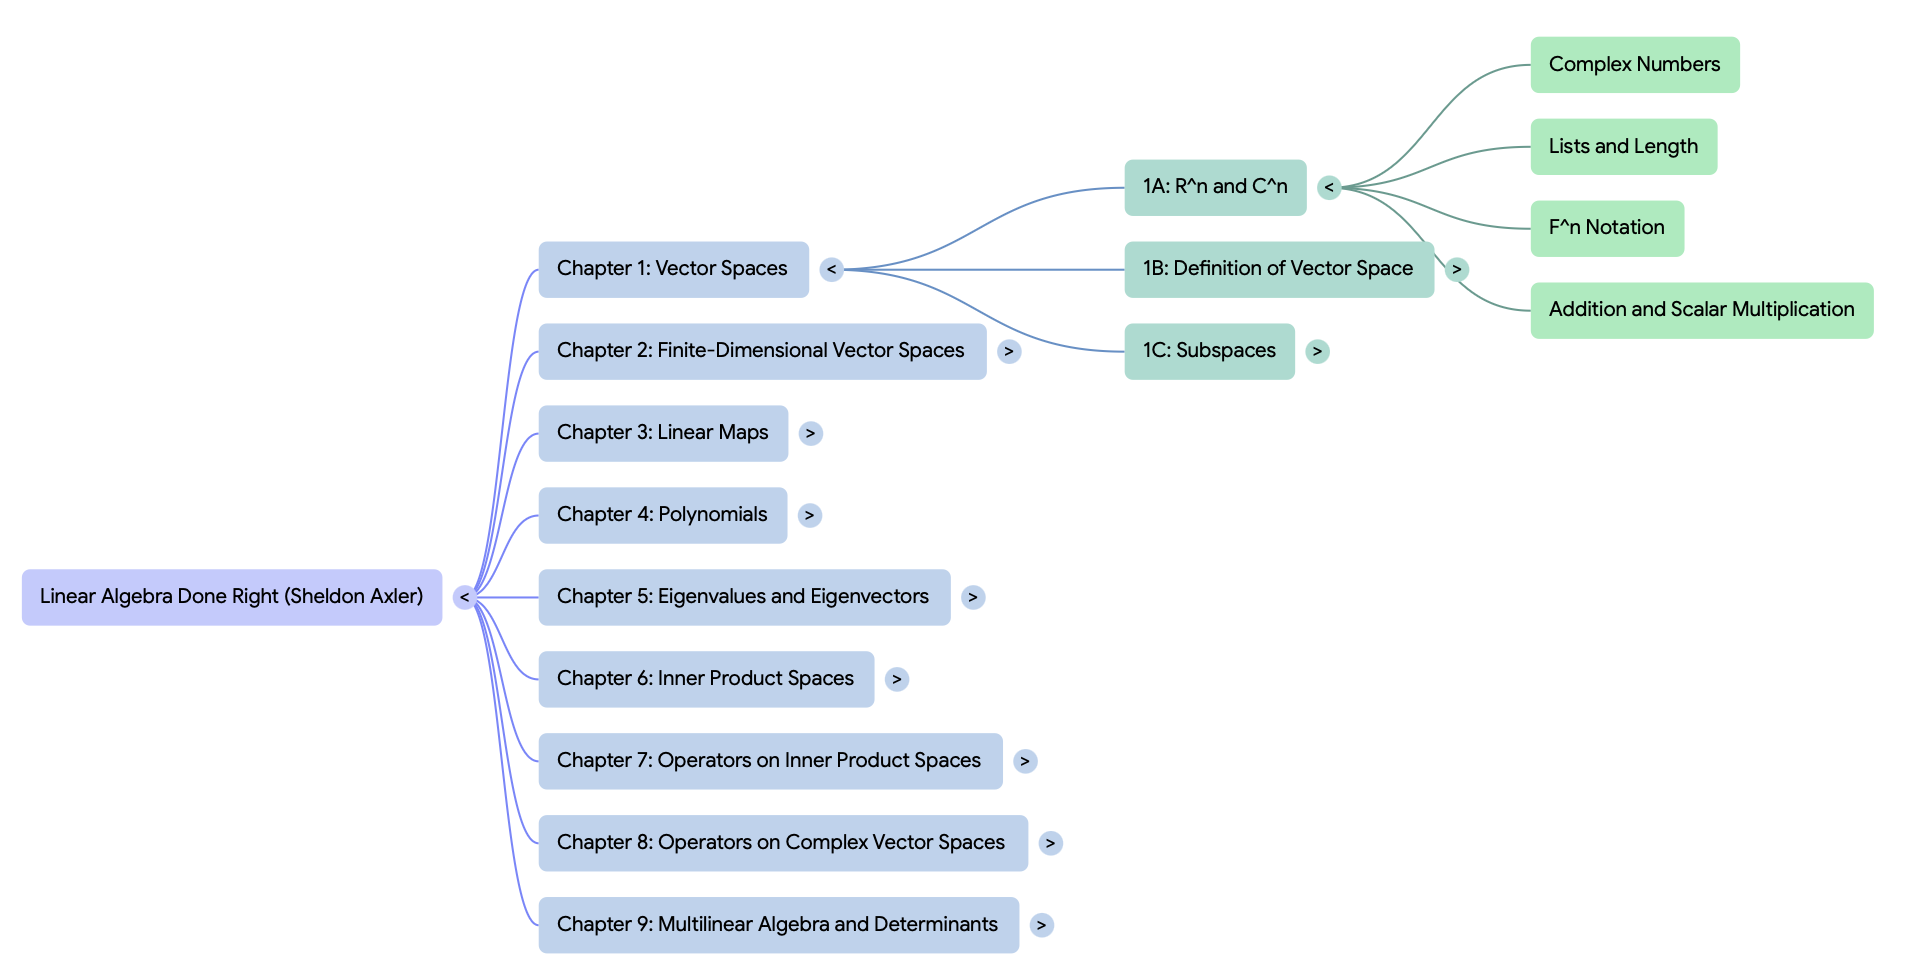
\includegraphics[width=\linewidth]{fig_notebooklm.png}\\[3pt]
  {\footnotesize (a) Google NotebookLM's mind-map view of the document,
   captured 27~August~2026. Edges denote containment; leaves are topic
   labels.}
\end{minipage}\hfill
\begin{minipage}[t]{0.47\textwidth}
  \centering
  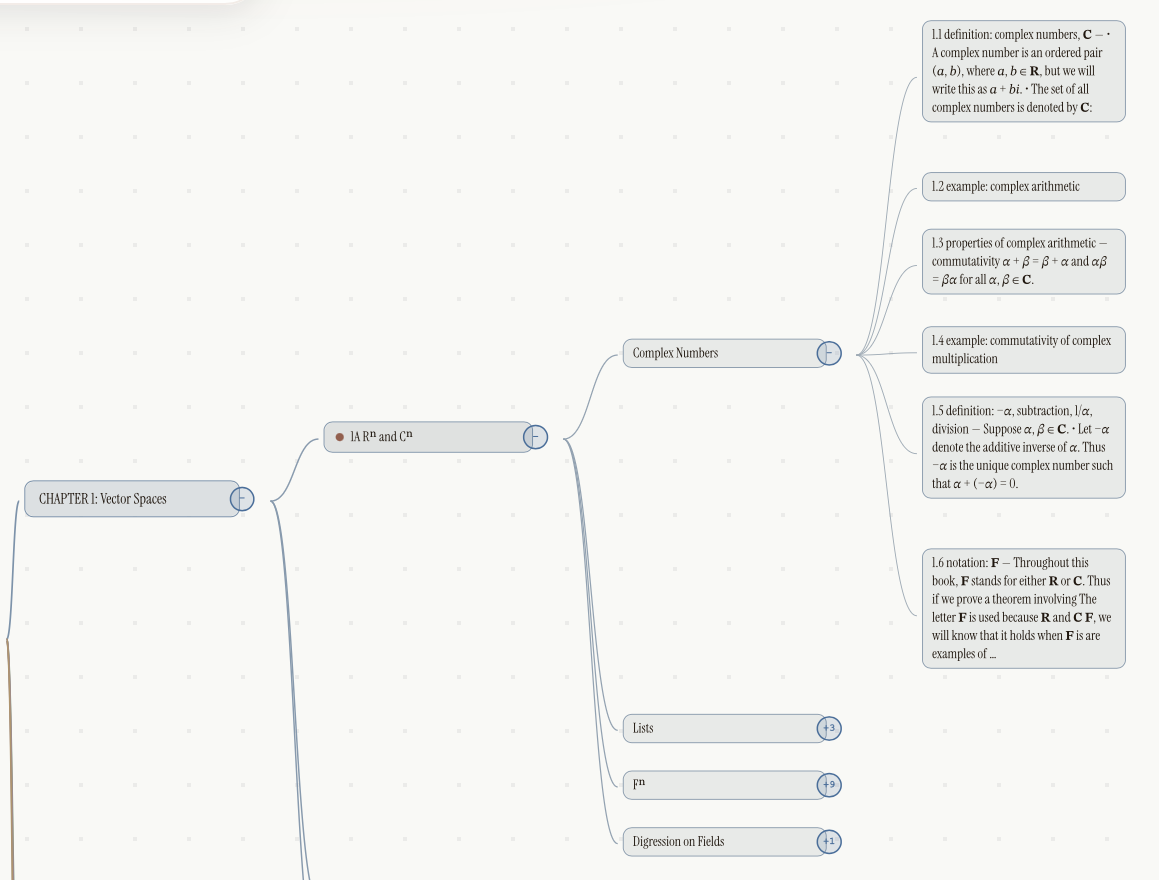
\includegraphics[width=\linewidth]{fig_tasur.png}\\[3pt]
  {\footnotesize (b) Tasur,\footnotemark[1] a prototype renderer, captured
   27~August~2026; one branch shown at full depth. Edges still denote
   containment, but the tree descends a level further, to typed atomic items
   retaining the source text and its notation.}
\end{minipage}

\vspace{8pt}
\begin{minipage}[t]{0.92\textwidth}
  \centering
  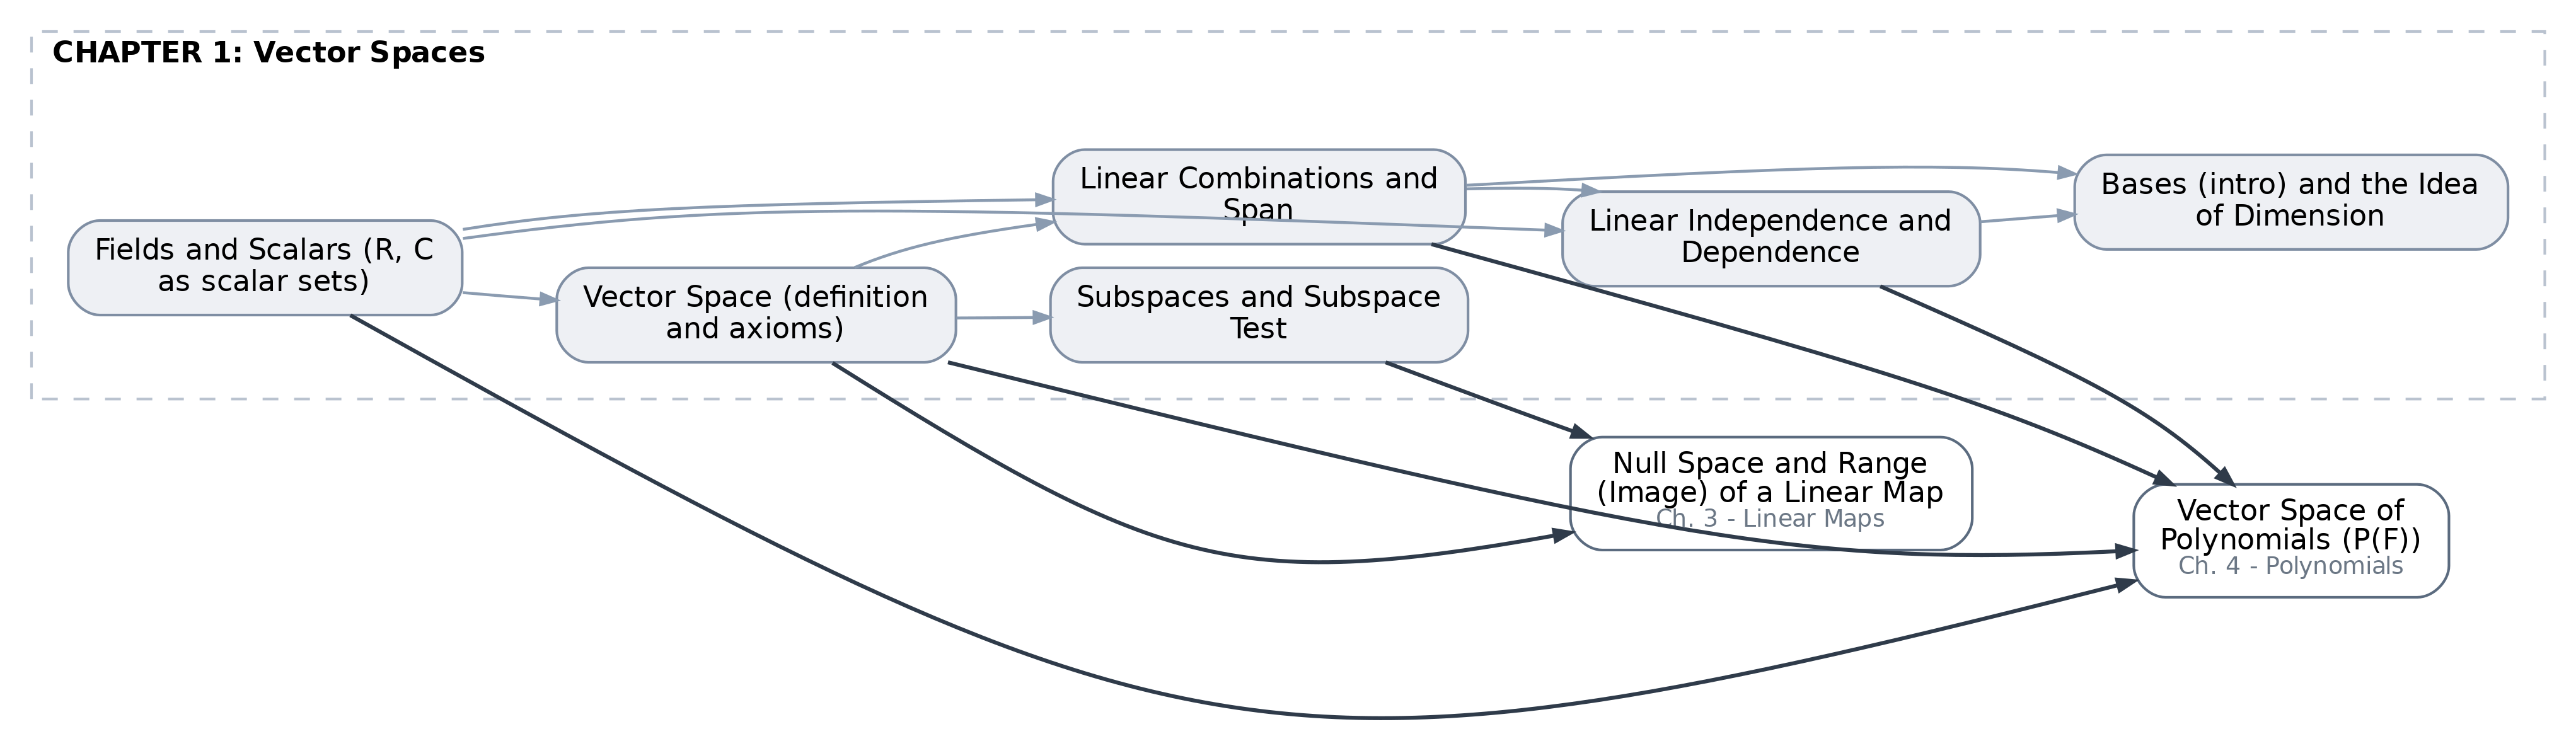
\includegraphics[width=0.95\linewidth]{fig_mard_graph.png}\\[3pt]
  {\footnotesize (c) MARD's compiled concept graph, drawn at the same scope and
   in the same visual idiom as (a) and (b) so that only \emph{edge semantics}
   differ. Chapter~1's six concepts, with the two dependents outside the
   chapter that they feed. Dark edges leave the chapter; grey edges stay
   inside it. Note what a containment tree cannot express: ``Vector Space of
   Polynomials'' has four prerequisites, all in Chapter~1, three chapters
   earlier. Full graph: 54 concepts, 116 edges, 76 of them cross-chapter.
   Single unreplicated run, seed 11.}
\end{minipage}

\caption{Three renderings of \emph{Linear Algebra Done Right}, 4th ed.,
the corpus document with the most explicit prerequisite structure and the
target of the dependency-ordering case study rather than the primary
measurement document. \textbf{All three were produced from an abridged
version of the text, not the full book.} Panels (a) and (b) differ in
resolution: both encode the containment hierarchy the document already
declares through its headings, and (b)---shown for a single branch, since at
whole-tree scale its leaves are illegible---descends a level further and
preserves mathematical notation. Panel (c) differs in kind: its edges
assert precedence rather than membership, and each is therefore a falsifiable
prediction rather than a restatement of the table of contents.}
\label{fig:trees}
\end{figure*}
\footnotetext[1]{Declaration of interest: Tasur is built and maintained by one
of the authors. It is included as an illustration of rendering granularity,
not as an evaluated system, and no performance claim is made for it in this
work. Neither named product is used as a quantitative baseline anywhere in
this paper, for the reasons given in Section~\ref{sec:related}: their
architectures are unpublished and they expose no token accounting, so no such
comparison would reproduce.}

\section{Methodology}
\label{sec:method}

\subsection{Design}
\label{sec:design}

\subsubsection{What the base library already provides}
\label{sec:baselib}
Formalising MARD requires first naming what it does not add, because the base
library ships a great deal that sounds like our contribution. Its metadata
types carry the root model, maximum depth, iteration count, backend and
environment; its completion object carries the full execution
trajectory---iterations, code blocks, and nested sub-calls, each with its own
metadata, recursively; and per-call token and cost accounting is built in.

That metadata, however, flows \emph{upward} and is observational: it is a
record of what happened, assembled for inspection after the fact. It never
re-enters a prompt and never influences a child call. This is checkable in
the source rather than a matter of framing. When a parent spawns a child, the
child is constructed with a fresh, empty logger---the library's own comment
says the purpose is that the child's trajectory be captured, not that the
parent's be communicated---and the child receives only the prompt string that
the parent's REPL code passed to it. Nothing else crosses the boundary.

MARD's envelope flows \emph{downward} and is operative. Skeleton, accumulated
findings and parent directive enter the child's context before it runs,
changing what the child can see and therefore what it produces.

One objection should be anticipated. The base library does expose a slot for
injecting a small user-authored string alongside the root's context, and
declines to populate it for children. The rebuttal is about what fills the
slot, not whether a slot exists: that parameter is designed for a fixed,
short, user-supplied string---its documentation's own example is the user's
original question. The envelope is accumulated state that grows across calls.
No mechanism in the base library constructs, propagates or compounds such
state, and none carries one child's findings to the next. The library gives
us somewhere to put an envelope; the envelope is ours.

\subsubsection{The metadata envelope}
Let $D$ be a document and $S(D)$ a \emph{skeleton}: an ordered structural
index of $D$'s chapters and sections with their positional spans, derived
from $D$'s own text. For a recursive call $c$ we define the envelope
\begin{equation}
E(c) = \bigl\langle\, S(D),\; F(c),\; d(c) \,\bigr\rangle ,
\end{equation}
where $F(c)$ is the set of findings accumulated by calls ordered before $c$,
and $d(c)$ is the directive issued by $c$'s parent stating the purpose of the
call. $E(c)$ is rendered into $c$'s prompt in addition to its text slice.

The design intent was that $E(c)$ remain small while $F(c)$ grows
monotonically with the number of completed calls: findings are summarised
rather than concatenated, and the rendering applies a recency window, so a
call sees the most recent findings rather than all of them---which predicts
that recovered cross-chapter relations will skew toward nearby chapters. An
earlier draft of this manuscript stated a per-call envelope budget of
approximately \num{300} tokens against a ceiling of \num{500}. Measuring the
rendered Pass~1 prompts directly refutes that figure, and we report the
measurement rather than the intent.

Across the \num{14} Pass~1 calls of a representative run, the skeleton
$S(D)$ renders at \num{4031} tokens---identical on every call, since it is
the same structural index---the accumulated findings $F(c)$ at a mean of
\num{1446} tokens and a maximum of \num{2853}, and the directive $d(c)$ at
\num{56}. The envelope is therefore on the order of \num{5500} tokens per
call against a total prompt of \num{5788}, and is not a small annotation
beside the text slice but the great majority of what the frontier tier reads.
The recency window does bound $F(c)$ as designed; the skeleton, which is not
subject to it, does not shrink at all.

This measurement anticipates the ablation result in
Section~\ref{sec:ablation}. The component consuming the most input is the one
whose removal costs nothing.

\subsubsection{Pass structure}
\label{sec:passes}

\begin{figure}[!t]
\centering
\scriptsize
\begin{tikzpicture}[
  font=\scriptsize,
  node distance=0pt,
  box/.style   ={draw, rounded corners=1pt, align=center, inner sep=3pt},
  doc/.style   ={box, dashed, draw=mardgrey, text=mardgrey,
                 text width=0.86\columnwidth},
  scoutbox/.style ={box, draw=mardblue, fill=mardbluebg, line width=0.5pt,
                 text width=0.90\columnwidth, inner ysep=4pt},
  swarmbox/.style ={box, draw=mardorange, fill=mardorangebg, line width=0.5pt,
                 text width=0.90\columnwidth, inner ysep=4pt},
  plan/.style  ={box, fill=mardink, draw=mardink, text=white,
                 text width=0.86\columnwidth, inner ysep=4pt},
  outbox/.style={box, draw=mardgrey, text width=0.86\columnwidth,
                 inner ysep=4pt},
  flow/.style  ={-{Latex[length=1.4mm]}, draw=mardgrey,
                 shorten >=1pt, shorten <=1pt}
]
% --- unbounded document -------------------------------------------------
\node[doc] (docnode)
  {\texttt{UNBOUNDED DOCUMENT} --- never loaded into any context};
\node[below=2.2mm of docnode, text width=0.86\columnwidth, align=center,
      inner sep=0pt, text=mardblue] (expose)
  {exposed as REPL environment variable};
\draw[flow] (docnode.south) -- (expose.north);
% --- tier 1: scout ------------------------------------------------------
\node[scoutbox, below=2.2mm of expose] (scout) {%
  \begin{minipage}{0.86\columnwidth}
  \centering
  \color{mardblue}%
  \makebox[\linewidth][s]{\texttt{TIER 1 --- THE SCOUT}\hfill
    frontier model $\cdot$ single session}\\[3pt]
  \begin{tikzpicture}[font=\scriptsize, cell/.style={draw=mardblue,
        fill=white, text=mardink, rounded corners=1pt,
        minimum height=4.5mm, align=center, inner sep=2pt}]
    \node[cell, text width=0.23\columnwidth] (p0) {Pass 0\\skeleton};
    \node[cell, text width=0.23\columnwidth, right=1.2mm of p0] (p1)
      {Pass 1\\exploration};
    \node[cell, text width=0.23\columnwidth, right=1.2mm of p1] (p2)
      {Pass 2+\\deep dive};
    \draw[-{Latex[length=1.2mm]}, draw=mardblue] (p0) -- (p1);
    \draw[-{Latex[length=1.2mm]}, draw=mardblue] (p1) -- (p2);
  \end{tikzpicture}\\[3pt]
  \color{mardblue}Envelope grows across passes $\cdot$ reads ${\approx}3$--$5\%$ of $D$
  \end{minipage}};
\draw[flow] (expose.south) -- (scout.north);
% --- master plan --------------------------------------------------------
\node[plan, below=2.2mm of scout] (plan)
  {\texttt{MASTER PLAN} --- concept graph $+$ ordered sequence\\
   (typed contract)};
\draw[flow] (scout.south) -- (plan.north);
% --- tier 2: builders ---------------------------------------------------
\node[swarmbox, below=2.2mm of plan] (swarm) {%
  \begin{minipage}{0.86\columnwidth}
  \centering
  \color{mardorange}%
  \makebox[\linewidth][s]{\texttt{TIER 2 --- THE BUILDERS}\hfill
    cheap model $\cdot$ $N$ in parallel}\\[3pt]
  
\begin{tikzpicture}[font=\scriptsize, cell/.style={draw=mardorange,
        fill=white, text=mardink, rounded corners=1pt,
        minimum height=4mm, minimum width=0.135\columnwidth, inner sep=1pt}]
    \node[cell] (b1) {$b_1$};
    \node[cell, right=1.1mm of b1] (b2) {$b_2$};
    \node[cell, right=1.1mm of b2] (b3) {$b_3$};
    \node[cell, right=1.1mm of b3] (b4) {$b_4$};
    \node[cell, right=1.1mm of b4] (bn) {$b_N$};
  \end{tikzpicture}\\[3pt]
  \color{mardorange}Wall-clock is $\max_i(b_i)$, not $\sum_i$ $\cdot$ join in plan order
  \end{minipage}};
\draw[flow] (plan.south) -- (swarm.north);
% --- output -------------------------------------------------------------
\node[outbox, below=2.2mm of swarm] (output)
  {\texttt{DEPENDENCY-ORDERED OUTPUT}};
\draw[flow] (swarm.south) -- (output.north);
\end{tikzpicture}
\caption{MARD architecture. The document is never placed in a prompt; it is
bound to a REPL variable and explored by the frontier tier, which emits a
typed Master Plan that dispatches a parallel budget tier. Pass~2 is specified
but \emph{not executed} in the configuration evaluated here
(Section~\ref{sec:passes}); the system reported in this manuscript is
two-pass.}
\label{fig:arch}
\end{figure}

MARD proceeds in passes over $D$, all executed by the frontier tier.
\begin{itemize}
  \item \textbf{Pass 0 --- skeleton extraction.} Derive $S(D)$ from the
  document's text. This pass is predominantly arithmetic over detected block
  structure rather than model inference; a single labelling call assigns
  topic labels. Crucially, the skeleton is text-derived only: where a source
  document ships a publisher-supplied bookmark outline, that outline is used
  solely as a yardstick for evaluating skeleton quality and is never an input
  (Section~\ref{sec:confounds}).
  \item \textbf{Pass 1 --- enriched exploration.} One call per chapter, each
  carrying $E(c)$ and each contributing to $F$. The output is the Master Plan.
  \item \textbf{Pass 2 --- targeted deep dive.} Revisit spans that Pass~1
  marked as uncertain, at greater depth.
\end{itemize}

\noindent\textbf{This manuscript reports a two-pass configuration.}
The system evaluated here executes Pass~0 and Pass~1 only; Pass~2 is not run.
This is stated here, in every results caption, and in the limitations,
because describing a two-pass system as three-pass would be an overclaim. The
decision was taken deliberately: Pass~1's implementation was completed one
day before this project's feature freeze, and the reliability of a pass
cannot be evidenced in a day. Layering a targeted deep dive on an unevidenced
exploration pass would make a subsequent wrong result undiagnosable---it
could not be attributed to either pass. The two-pass configuration is
additionally, and by design, the depth-0 point of the depth sweep in
Section~\ref{sec:ablation}, so this manuscript's number is a valid point on
that curve rather than a one-off compromise.

\subsubsection{The Master Plan as a typed contract}
Pass~1 emits a \emph{Master Plan}: a concept graph together with an ordered
study sequence and the rationale for any reordering. It is validated against
a schema at the tier boundary, and a malformed plan fails loudly rather than
dispatching $N$ subtly incorrect builders.

The field that carries the contribution is the concept graph's edge set. Each
edge asserts that one concept is prerequisite to another, and each is
therefore a falsifiable prediction scorable against the document's own
in-text cross-references. Edges are validated at the boundary: an edge naming
a concept that no call has declared is rejected and logged rather than
silently admitted, which makes the rejection log itself a measurement of what
exploration could and could not reach.

\subsubsection{Two-tier execution and dependency-ordered joining}
The Scout (frontier tier, single session) reads approximately 3--5\% of $D$
and emits the Master Plan. The Swarm (budget tier) then runs $N$ builders in
parallel, one per section, each receiving its section slice plus its plan
directive. Because the builders fork and join, wall-clock time is
$\max_i(\mathrm{builder}_i)$ rather than $\sum_i$, and we report both so that
the parallelism claim is checkable rather than asserted.

Builder outputs are joined in Master Plan order---the dependency-derived
ordering---rather than in book order. We note explicitly that book order is
itself an expert baseline, since the document's author already sequenced the
material; reordering must therefore beat a real ordering, not a random one.
The join additionally validates non-empty output per plan step and raises
rather than returning a partial artefact, so a run that produced a short
result fails visibly instead of scoring as a complete but poor one.

\subsubsection{What MARD changes, and what it inherits}
\label{sec:comparison}
Table~\ref{tab:arch} sets the two arms side by side. It is grouped deliberately: the
upper block is what MARD takes unchanged from the base paper, and only the lower
block is ours. Presenting the comparison the other way round---differences
first, shared machinery unstated---would let a reader credit MARD with the
recursion and the tiering, which are not our contribution
(Section~\ref{sec:baselib}).

\begin{table*}[!t]
\caption{Architectural Comparison of the Two Arms. Both Run on One
Implementation, at Matched Recursion Depth, on Identical Inputs. The Upper
Block is Inherited from the Base Paper and is Not Claimed as a Contribution}
\label{tab:arch}
\centering
\renewcommand{\arraystretch}{1.25}
\begin{tabular}{@{}p{3.5cm}p{6.0cm}p{6.4cm}@{}}
\toprule
\textbf{Aspect} & \textbf{Vanilla RLM (B1)} & \textbf{MARD} \\
\midrule
\multicolumn{3}{@{}l}{\textbf{Inherited from the base paper --- identical in both arms, and not our contribution}} \\
\midrule
Document placement & Bound to a REPL variable; never enters a prompt & Identical \\
Model tiering & Frontier root, budget sub-calls & Frontier Scout, budget Swarm --- the same economics \\
Recursion depth & Sub-calls are plain completions & Matched, by construction \\
Input & Cleaned text stream; front matter excluded, publisher outline withheld & Identical, by construction \\
\midrule
\multicolumn{3}{@{}l}{\textbf{Where MARD differs}} \\
\midrule
Exploration strategy & Authored at run time by the root model as REPL code & Fixed pass structure; the model supplies findings, not control flow \\
Structural map & None. Any structure must be re-derived by code the root writes & Pass~0 skeleton, derived from the document's own text \\
What a sub-call receives & A raw text slice & Slice \emph{plus} skeleton, accumulated findings, and a parent directive \\
State across calls & None; each sub-call is independent & Envelope accumulates; a later chapter sees earlier chapters' findings \\
Direction of metadata & Upward, observational --- recorded after the fact & Downward, operative --- enters the prompt before the call runs \\
Unit of dispatch & Chosen by the root at run time & Chapter for exploration; section for generation \\
Intermediate artefact & None; free text inside the root's own history & Typed Master Plan: concept graph, ordered sequence, reordering rationale \\
Source binding at generation & The model matches text to a concept at generation time & The brief is constructed from the plan's recorded source span \\
Output ordering & Whatever the root emits & Master Plan order, i.e.\ dependency order \\
Malformed intermediate & No intermediate to validate; execution proceeds & Schema validation at the tier boundary; a malformed plan fails loudly \\
Empty generation & Included in the output; run reports success & Join validates non-empty text per plan step and raises \\
Parallelism & As the root's code chooses & $N$ builders fork--join; wall-clock is $\max_i$, not $\sum_i$ \\
\bottomrule
\end{tabular}
\end{table*}

Three rows in the lower block are worth reading together, because they describe
a single property rather than three. \emph{Source binding}, \emph{malformed
intermediate} and \emph{empty generation} are the points at which MARD can
refuse to proceed. Vanilla RLM has no equivalent of any of them: it has no
typed intermediate to validate, and no record of which span a given concept
should have been written from, so there is nothing against which a generation
step could be checked. That asymmetry is the mechanism behind the
faithfulness observation reported in Section~\ref{sec:grounding}, and it is
architectural rather than incidental.

\subsubsection{The stated precondition}
\label{sec:precondition}
MARD requires exploitable structure. On a flat context there is no skeleton
to extract, $F$ carries no positional meaning, and the envelope reduces to
overhead. We therefore predict that MARD degenerates to vanilla-RLM behaviour
on flat inputs, and we test this with a negative control rather than omitting
it. This is an objective of the work, not an embarrassment to be discovered
in review.

The control is a \emph{structure-ablated variant of the primary document}: the
same text with its section order shuffled and its heading markers removed.
This is a deliberate choice over an external flat-context benchmark. It holds
content constant and varies only structure, so it is a manipulation rather
than a change of corpus, and it parallels the envelope ablation one level
lower---A1 removes the accumulated structure the system builds, and this
removes the structure the document supplies. The pipeline treats the resulting
empty skeleton as a recorded condition rather than an error, so degeneration
appears in the run log as a finding rather than as a missing value. An
external flat-context benchmark subset is fixed and frozen in the project's
evaluation artefacts and is run in the full study
(Section~\ref{sec:future}).

\subsection{Algorithm and Implementation}
\label{sec:impl}
\label{sec:setup}

\subsubsection{The algorithm}
Algorithm~\ref{alg:mard} states MARD end to end. Three lines carry properties
argued for elsewhere in this section and are worth reading as such. Line~3 is
the boundary condition of Section~\ref{sec:precondition}: a document from
which no skeleton can be derived returns a recorded degenerate condition
rather than an error, so graceful degeneration appears in the run log as a
finding. Line~9 is the validation boundary---an edge naming a concept no call
has declared is rejected and logged, which makes the rejection log itself a
measurement of what exploration could not reach. Line~16 is the source
binding: a builder's brief is constructed from the plan's recorded span, so
generation never depends on a model matching text to a concept.

\begin{algorithm}[!t]
\caption{MARD (two-pass configuration)}
\label{alg:mard}
\begin{algorithmic}[1]
\REQUIRE document $D$ with section index; frontier model $M_1$; budget model $M_2$
\ENSURE dependency-ordered artefact, or a loud failure
\STATE $K \leftarrow \textsc{Skeleton}(D)$ \COMMENT{Pass 0; text-derived only}
\IF{$K = \emptyset$}
  \RETURN \textsc{Degenerate} \COMMENT{O4 boundary; recorded, not an error}
\ENDIF
\STATE $E \leftarrow \textsc{Envelope}(K,\ F {=} \emptyset,\ d {=} \textbf{nil})$
\FOR{each chapter $c \in K$ \textbf{in book order}}
  \STATE $E_c \leftarrow E.\textsc{ForChild}(c,\ \textsc{Directive}(c))$
  \STATE $R \leftarrow M_1(\textsc{Render}(E_c) \,\Vert\, \textsc{Text}(c))$ \COMMENT{Pass 1}
  \STATE $C_c, X_c \leftarrow \textsc{Validate}(R,\ \textsc{Known})$ \COMMENT{reject undeclared}
  \STATE $E \leftarrow E.\textsc{WithFindings}(c,\ C_c,\ X_c)$ \COMMENT{envelope grows}
\ENDFOR
\STATE $P \leftarrow \textsc{CompilePlan}(C,\ X,\ K)$ \COMMENT{typed Master Plan}
\IF{$P$ fails schema validation}
  \STATE \textbf{fail loudly} \COMMENT{never dispatch on a malformed plan}
\ENDIF
\STATE $B \leftarrow \textsc{BriefsFor}(P)$ \COMMENT{each brief carries $P$'s recorded span}
\FORALL{$b \in B$ \textbf{in parallel}}
  \STATE $s_b \leftarrow M_2(\textsc{Prompt}(b))$ \COMMENT{Tier 2; wall-clock $\max_i$}
\ENDFOR
\IF{any $s_b$ is empty}
  \STATE \textbf{raise} \textsc{IncompleteArtefact}
\ENDIF
\RETURN $\textsc{Join}(\{s_b\},\ P.\textsc{sequence})$ \COMMENT{plan order, not book order}
\end{algorithmic}
\end{algorithm}

\subsubsection{Model pair, parity and cost}
The frontier tier (Scout) is \texttt{gpt-5.2}; the budget tier (Swarm, and the
baseline's sub-calls) is \texttt{gpt-5-mini}. Rates were read from the
provider's own pricing page on the day the rate card was written and are
recorded once, in code, with their source and retrieval date; the accounting
layer refuses to price a run against a rate more than thirty days old rather
than let a stale figure ride.

We are explicit that this pair is selected on \emph{role fit and cost}, not on
a published benchmark comparison. The Scout runs once per document and must
hold the skeleton and accumulated envelope across a sequence of chapter calls;
the Swarm is $N$ independent builders each consuming one section and a
directive, where call volume rather than per-call ceiling dominates. The
budget tier carries roughly 93\% of the token volume at approximately one
seventh the rate on both input and output. A model sweep that would test that
reasoning is deferred to the full study, and we do not present the selection
as a measured result.

\noindent\textbf{Both arms are executed on a single implementation.}
Isolating the envelope requires that the two arms differ \emph{only} in its
presence. Executing the baseline on a separate codebase would confound the
envelope with two independent implementations---differing prompt templates,
REPL surfaces and stopping criteria---none of which is the variable under
study. We therefore implement vanilla RLM as an envelope-disabled
configuration of the same system, and treat the reference implementation
accompanying the base paper \cite{zhang2025rlm} as the specification we
implement against rather than as the artefact we measure.

The cost of this choice is that our baseline is our own implementation of RLM
rather than the original authors'. We mitigate it in the only way available:
by reproducing a published result from the base paper first-hand on our own
harness before any number in Section~\ref{sec:results} is trusted. That check
is not a formality here---it is the sole evidence that the vanilla arm
faithfully reproduces the published method.
\textbf{This check was not performed.} The provider migration described in
Section~\ref{sec:setup} consumed the time allocated to it, and we report its
absence rather than substituting a weaker check and calling it done. The
consequence is stated plainly: we have no first-hand evidence that our vanilla
arm reproduces the published method's performance, only that it implements the
published method's mechanism, which our tests assert directly. Every
comparison in Section~\ref{sec:results} should be read as against
\emph{our implementation of} RLM. This is the single largest threat to the
baseline's validity in this manuscript and it is unresolved.

What we did run is a bounded harness check, and we are careful about what it
does and does not establish. Six tasks from the frozen OOLONG subset were
executed end to end through the vanilla arm and scored with the base paper's
own scoring function, imported unmodified from the reference implementation
rather than reimplemented. All six executed, and all six produced output the
reference scorer could parse. \textbf{We report no accuracy estimate from six
tasks and draw no comparison to the published figure}---at that sample size the
confidence interval spans both the published RLM result and the base model's,
so a number would carry the appearance of evidence without its substance. What
the check rules out is narrow and worth stating anyway: the failure mode in
which our harness cannot execute the published benchmark at all, or emits
output the reference metric cannot read. It leaves the paragraph above
unchanged.

\noindent\textbf{Concurrency and sub-call size are bounded, identically for
both arms.}
Runs were executed under a provider rate-limit tier that required bounding
sub-call concurrency and sub-call input size.
Sub-call concurrency was bounded at $4$ simultaneous calls, and Tier~2
generations at $4{,}096$ completion tokens with reasoning effort set to
\texttt{low}---the latter after $15$ of $84$ builders in an early run spent an
entire $2{,}048$-token budget on reasoning and returned empty artefacts, which
the typed join surfaced as an error rather than as a short document.
Both bounds are applied to \emph{both} arms and are recorded in every run's
configuration snapshot. We report this because it is not a neutral
implementation detail: throttling can degrade output completeness, and
applying it asymmetrically would manufacture a difference between the arms
that has nothing to do with the envelope.

The cost model is instantiated with measured token counts rather than a
claimed multiple. Table~\ref{tab:cost} reports the projected cost of the full
evaluation matrix from measured corpus quantities. We report the model rather
than a headline ratio because provider rates move month to month, and a fixed
multiple quoted against a rate that later disappears is precisely the kind of
claim that decays into misinformation.

\begin{table}[!t]
\caption{Cost of the Evaluation Matrix on the Primary Document. Corpus
Quantities and the Baseline's Per-Run Cost are Measured; the MARD Figure is
Projected from Those Quantities at the Same Rates}
\label{tab:cost}
\centering
\renewcommand{\arraystretch}{1.2}
\begin{tabular}{@{}p{5.0cm}R{2.2cm}@{}}
\toprule
\textbf{Measured quantity} & \textbf{Value} \\
\midrule
Primary document, characters        & 2\,468\,431 \\
Primary document, tokens\textsuperscript{\dag} & $\approx$617\,000 \\
Sections (Swarm builders)           & 120 \\
Chapters explored by Pass~1         & 14 \\
\midrule
\multicolumn{2}{@{}l}{\textbf{Published rates, per \num{1000000} tokens}} \\
Frontier tier, input / output       & \$1.75 / \$14.00 \\
Budget tier, input / output         & \$0.25 / \$2.00 \\
\midrule
\multicolumn{2}{@{}l}{\textbf{Cost per run}} \\
Vanilla RLM, measured\textsuperscript{\ddag} & \$0.32--\$1.60 \\
MARD, projected                     & $\approx$\$0.94 \\
\midrule
Remaining matrix, projected         & $\approx$\$11 \\
\bottomrule
\end{tabular}
\vspace{2pt}
\begin{minipage}{\columnwidth}
\footnotesize \textsuperscript{\dag}Derived from character counts at an
assumed ratio; pending confirmation with a tokeniser.
\textsuperscript{\ddag}Three logged runs; the spread is reported rather than
averaged, for the reason given in Section~\ref{sec:variance}.
\end{minipage}
\end{table}

\subsubsection{Corpus and licensing}
Our corpus consists of openly licensed textbooks spanning distinct domains,
under an open-license-only constraint on all source material.
Table~\ref{tab:corpus} summarises them. Licensing was verified against each
publisher's own copyright page rather than a third-party aggregator.

\begin{table}[!t]
\caption{Corpus Documents and Licences, Verified Against Each Source's Own
Copyright Page}
\label{tab:corpus}
\centering
\renewcommand{\arraystretch}{1.2}
\begin{tabular}{@{}p{3.5cm}p{2.4cm}p{1.4cm}@{}}
\toprule
\textbf{Document} & \textbf{Licence} & \textbf{Role} \\
\midrule
Introduction to Computer Science (OpenStax) & CC BY 4.0 & Primary \\
University Physics, Vol.~1 (OpenStax) & CC BY-NC-SA 4.0 & Secondary \\
Linear Algebra Done Right, 4th ed. & CC BY-NC 4.0 & Secondary \\
\bottomrule
\end{tabular}
\end{table}

OpenStax titles were selected specifically because they ship
machine-readable learning objectives, glossaries and answer keys---the
substrate required for document-native ground truth extracted without human
annotation, and therefore without an ethics-approval process this project's
timeline cannot absorb.

\noindent\textbf{On the licence of the primary document.}
\emph{Introduction to Computer Science} is CC BY 4.0 (plain attribution),
confirmed against OpenStax's book-level licensing page. Individual chapter
footers within the same book state CC BY-NC-SA; we treat the book-level page
as authoritative and record the inconsistency rather than silently choosing
one.

\subsubsection{Ingestion and primary-document selection}
Primary-document selection was made on measured evidence rather than
convenience. Table~\ref{tab:parse} reports parse quality across the three
candidates. No optical character recognition is used on any document: all
three carry a text layer, and OCR would replace exact text with approximate
text---decisively, OCR errors in glossary terms would corrupt the very
reference set against which task quality is scored, silently and
irreversibly.

\begin{table}[!t]
\caption{Parse Quality, Produced by the Ingestion Pipeline and Reproducible
from the Corpus Artefacts. Orphan Punctuation Counts Punctuation Stranded
Where a Formula Failed to Extract}
\label{tab:parse}
\centering
\renewcommand{\arraystretch}{1.2}
\begin{tabular}{@{}p{3.2cm}R{1.05cm}R{1.05cm}R{0.95cm}@{}}
\toprule
\textbf{Measure} & \textbf{introcs} & \textbf{physics1} & \textbf{axler} \\
\midrule
Pages                              & 939       & 959       & 404 \\
Characters after cleaning          & 2\,432\,812 & 2\,032\,210 & 737\,844 \\
Headings detected                  & 1\,403    & 1\,081    & 17 \\
Learning-objective blocks          & 61        & 99        & 0 \\
Key-terms blocks                   & 14        & 17        & 0 \\
Orphan punctuation (per 1k lines)  & 30.3      & 113.5     & 87.8 \\
Warnings raised                    & 0         & 1         & 3 \\
\bottomrule
\end{tabular}
\end{table}

\emph{University Physics} is disqualified as primary on content loss, not
formatting loss: its orphan-punctuation rate is nearly four times that of the
primary document, and inspection confirms sentences from which equations have
vanished entirely. That damage is not uniform across systems under test---a
configuration that reads more of the document encounters more of it---and
would manufacture a difference between MARD and vanilla RLM having nothing to
do with either. \emph{Linear Algebra Done Right} carries no learning
objectives and no key-terms sections, so document-native ground truth cannot
be extracted from it; it remains the strongest candidate for the
dependency-ordering case study, which is scored separately.

Page mapping was verified by sampling \num{1200} blocks at random across the
three documents and confirming each appears on the page it claims;
\num{1199} passed, the single failure being a whitespace-normalisation
difference in an index line rather than a mapping error.

\subsubsection{Two structural confounds, and how they are controlled}
\label{sec:confounds}
Both concern structure reaching a model without that model having derived it.
If structure arrives by another route, we would be reporting the publisher's
work as MARD's.

\begin{enumerate}
  \item \textbf{The publisher's bookmark outline.} All three documents ship
  one. The ingestion pipeline writes it to a separate artefact with an
  explicit provenance field and never merges it into the text stream, so that
  using it must be a deliberate decision rather than an accident. It serves as
  the yardstick for skeleton quality and is not an input to Pass~0.
  \item \textbf{The printed table of contents inside the body text.} Subtler,
  because it arrives through the ordinary text channel: the primary document
  prints its full chapter list on page~7, so a model reading the opening pages
  obtains the skeleton for free. Front matter is detected, tagged, and
  excluded from the text stream supplied to every system.
\end{enumerate}

Both controls are applied identically to the vanilla-RLM arm. If the two arms
received different inputs, the comparison would not isolate the envelope.

\subsubsection{Skeleton fidelity}
Because the skeleton is the substrate for everything downstream, its quality
is measured before it is used. Against the publisher outline, the primary
document's text-derived skeleton achieves \SI{82.2}{\percent} recall at
\num{0.0} pages of boundary error. Boundary error of zero indicates that
where a section is recovered, its span is recovered exactly; the recall
shortfall is missed sections, not misplaced ones.

\subsubsection{Systems compared}
\begin{itemize}
  \item \textbf{MARD} --- two-pass, as specified above.
  \item \textbf{B1, vanilla RLM} --- the isolation baseline: the base paper's
  architecture, a root REPL loop issuing flat sub-calls, on identical models,
  document and structural controls.
  \item \textbf{A1, envelope removed} --- MARD's architecture with the
  envelope emptied. This is a \emph{separate} run from B1 and serves a
  different purpose, discussed below.
  \item \textbf{Negative control} --- MARD and B1 on the structure-ablated
  variant of the primary document, testing the graceful-degeneration half of
  the claim under content held constant.
\end{itemize}

B1 and A1 are deliberately distinguished, because they answer different
questions. B1 compares MARD's architecture against the base paper's, and a
win there changes several things at once---the envelope, the pass structure,
the typed plan, two-tier dispatch and dependency-ordered joining. A1 holds
the architecture fixed and removes only the envelope, and is therefore the
only comparison that attributes an effect to the envelope specifically, which
is what this paper's claim rests on. Reporting B1 alone would license the
weaker conclusion that our pipeline is better, not that the envelope is why.

The full study additionally runs full-context, naive chunking and
embedding-RAG baselines first-hand.

\noindent\textbf{Recursion depth is held fixed.}
Both arms run at a matched recursion depth in which sub-calls are plain
completions. This is the base paper's primary reported condition. Holding
depth fixed is not incidental: if the arms differed in depth, the measured
difference would confound the envelope with an extra layer of recursion, and
the isolation claim would be void.
We resolve the correspondence architecturally, and disclose that the run logs
do not independently confirm it. The control arm runs at
\texttt{max\_depth}~$=1$: a root call plus one level of delegated sub-calls.
MARD's Tier~1 Scout issues one Pass~0 labelling call and one exploration call
per chapter, and dispatches Tier~2 builders; this is likewise one level of
delegation, fixed by the architecture rather than configurable, which is why
MARD's configuration snapshot records no depth parameter. The two arms
therefore match on the property that matters---neither nests delegation more
than one level deep.

The disclosure is that MARD's call log records every call at depth~\num{0},
including all \num{84} Tier~2 builders, and \texttt{parent\_call\_id} is
unpopulated in both arms. The control arm does distinguish its root from its
sub-call. A reader cannot therefore verify the depth match from the logs alone,
only from the call roles and the source; the correspondence above rests on the
latter. This does not satisfy our own measurement protocol, which requires
depth to be recorded as an \texttt{(enable\_sub\_calls,
max\_recursion\_depth)} pair precisely so that a matched-depth claim is
checkable rather than asserted. We record it as an instrumentation defect
found during manuscript preparation and not repaired before the results
freeze.

\subsubsection{Metrics}
Every run of every system records the fields in Table~\ref{tab:fields}. A
number that cannot be traced back to all of them from a logged run is not
admitted to this paper.

\begin{table}[!t]
\caption{Recorded Per Run. A Number Not Traceable to All of These From a
Logged Run is Not Admitted}
\label{tab:fields}
\centering
\renewcommand{\arraystretch}{1.2}
\begin{tabular}{@{}p{2.2cm}p{5.6cm}@{}}
\toprule
\textbf{Field} & \textbf{Definition} \\
\midrule
Task score & Explanation quality against document-native ground truth \\
Tokens & Input and output, summed over every model call, logged separately \\
Calls issued & Split by tier \\
Cost & At the same-day published provider rate \\
Wall-clock & Both $\max_i$ and $\sum_i$ over builders, so the parallelism claim is checkable \\
Run identifier & System, document, repeat \\
Config snapshot & Model identifiers, prompt-template versions, depth, active ablation, document, library revision \\
\midrule
\multicolumn{2}{@{}l}{\textbf{Additionally, for systems producing per-concept output}} \\
\midrule
Groundedness rate & Grounded concepts as a fraction of the total (Section~\ref{sec:grounding}) \\
Regenerations & Concepts with $\geq$1 discarded prior attempt \\
\bottomrule
\end{tabular}
\end{table}

\noindent\textbf{Task score.}
The evaluated output modality is explanations only. Flashcards, quizzes and
diagrams are demonstrable prototype features that test nothing about the
envelope and would multiply the evaluation surface; they are excluded from
measurement. Explanations are scored against document-native ground truth
extracted programmatically. Of the ground-truth sources available in the
corpus, this manuscript uses \emph{per-chapter learning objectives} and
\emph{in-text cross-references}. Glossary terms are present in the corpus but
are typeset as an undelimited run-on list, and recovering term boundaries
reliably requires font-level information we defer to the full study; they are
therefore \emph{not} used here. We state this because a restriction disclosed
is a scope decision and a restriction implied is not.
Matching is stemmed token-set overlap, scored as recall of the objective's
content tokens against the candidate explanation, with stopwords and tokens
under three characters removed. The reported threshold is $0.6$; every figure
is additionally computed at $0.5$ and $0.7$ and the ranking of configurations
is unchanged at all three. Raw matched and reference token counts are retained
per objective in the results log, so a reviewer who rejects the threshold can
recompute from the same artefacts without an API key. Scores are computed
per chapter and objective-weighted, not over the whole document: at
whole-document granularity every configuration scores between $0.94$ and
$0.97$ and the metric does not discriminate.

\noindent\textbf{Dependency-ordering score.}
Scored independently of task quality, as forward-reference violations: the
number of times a generated sequence places a concept before something the
document itself declares as its prerequisite, counted for book order and for
Master Plan order.

\noindent\textbf{Variance.}
Every reported number is the result of three independent repeated runs, with
spread reported alongside the central value. We report repeats rather than
fixed random seeds deliberately: the inference endpoints used here do not
expose deterministic decoding, so a nominal seed would name a property the
system does not have. Where variance swamps an effect, that is reported as
the finding.

\section{Results and Discussion}
\label{sec:results}
% >>> PENDING: no number in this section is real yet. Nothing may be written
% here that does not trace to a logged run. After the results freeze, numbers
% are written up and never re-run; a wrong result receives a limitation
% paragraph, not a second attempt.

\subsection{Isolating the envelope}
Table~\ref{tab:main} reports the four configurations on the primary document,
three repeated runs each, at matched recursion depth. Task score is
objective-weighted per-chapter coverage of the document's own learning
objectives at a stemmed-overlap recall threshold of $0.6$
(Section~\ref{sec:method}); the two neighbouring thresholds are reported
in the supplementary results log, and the ranking is stable across all three.

The frozen ablation set specified A1 as ``the envelope removed.'' We report it
as two separable manipulations, because the envelope carries two distinct
channels: the \emph{skeleton}, a structural map of the document, and the
\emph{accumulated findings}, the record of what earlier chapters established.
A1s suppresses the skeleton; A1f suppresses the findings. Reporting them
separately is what makes the result in Section~\ref{sec:ablation} legible.

\begin{table}[!t]
\caption{The Four Configurations on the Primary Document. Three Repeated Runs
Each; Mean With Min--Max in Parentheses. No Repeat Was Excluded}
\label{tab:main}
\centering
\renewcommand{\arraystretch}{1.2}
\begin{tabular}{@{}p{2.35cm}R{1.75cm}R{1.75cm}R{1.35cm}@{}}
\toprule
\textbf{System} & \textbf{Task score} & \textbf{Input tok.} & \textbf{Cost} \\
\midrule
B1, vanilla RLM & 0.551 \newline (0.315--0.765) & 1{,}493{,}033 \newline (517k--3{,}315k) & \$0.832 \newline (0.32--1.60) \\
MARD (two-pass) & 0.621 \newline (0.584--0.650) & 94{,}242 \newline (93.8k--94.7k) & \$0.578 \newline (0.57--0.59) \\
A1s, skeleton suppressed & 0.730 \newline (0.720--0.745) & 37{,}631 \newline (36.4k--38.6k) & \$0.498 \newline (0.49--0.50) \\
A1f, findings suppressed & 0.623 \newline (0.560--0.658) & 78{,}064 \newline (77.5k--78.6k) & \$0.524 \newline (0.51--0.53) \\
\bottomrule
\end{tabular}
\end{table}

MARD's mean task score exceeds the baseline's by $0.070$, and its mean input
token count is $15.8\times$ lower. Neither figure supports a claim that MARD
produces better explanations. The baseline's best repeat scores $0.765$,
above MARD's best of $0.650$; with three repeats and ranges that overlap this
far, the difference in means is not a difference we can defend. We state the
task-score comparison as \textbf{indistinguishable}, and locate the
contribution elsewhere.

The token reduction requires a similar qualification. MARD's Tier~2 builders
receive a concept label, a section identifier and a page range, and never the
document's prose (Section~\ref{sec:design}). Part of the $15.8\times$
reduction is therefore attributable to MARD not reading the text at the point
of generation, rather than to reading it more efficiently. We report the
reduction as a property of the architecture as specified, not as evidence of
superior retrieval, and return to it in Section~\ref{sec:threats}.

\subsection{Variance across repeats}
\label{sec:variance}
The spread in Table~\ref{tab:main} is the result. Under identical
configuration on an identical document, the baseline's task score ranges from
$0.315$ to $0.765$---a spread of $0.450$, or $82\%$ of its own mean. MARD's
ranges from $0.584$ to $0.650$, a spread of $0.066$. The baseline's input
token count varies by a factor of $6.4$ across the same three repeats
($517{,}000$ to $3{,}315{,}000$); MARD's varies by $0.9\%$. Its cost varies
$5.0\times$; MARD's by $3.8\%$.

This instability is visible in the artefacts themselves. Table~\ref{tab:struct}
reports the organisational structure each system imposed. The baseline emitted
$156$, $190$ and $75$ concept-level sections on its three repeats, and its
chapter-level organisation shifted from $20$ headings, to none at all, to a
single one. MARD emitted $84$, $83$ and $84$ concepts, each carrying a
verified section identifier and page range.

\begin{table}[!t]
\caption{Structural Stability and Provenance, Three Repeats Each. Concept
Counts Are Post-Merge; Duplicate Declarations Are Merged Rather Than
Rejected. Citations Are Source References That Resolve Against the Corpus}
\label{tab:struct}
\centering
\renewcommand{\arraystretch}{1.2}
\begin{tabular}{@{}p{2.5cm}R{2.4cm}R{1.05cm}R{1.05cm}@{}}
\toprule
\textbf{System} & \textbf{Concepts / sections} & \textbf{Ch. cov.} & \textbf{Cites} \\
\midrule
B1, vanilla RLM & 156, 190, 75 & 14, 14, 9 & 0, 0, 0 \\
MARD (two-pass) & 84, 83, 84 & 14, 14, 14 & 84, 83, 84 \\
\bottomrule
\end{tabular}
\end{table}

Two properties follow, and we are careful to distinguish them. MARD's
\emph{scaffold} is near-deterministic: the concept set is computed from a
skeleton derived from the verified corpus rather than sampled, and varies only
where a duplicate-identifier merge fires. Its \emph{elaboration} is not: edge
counts range $124$--$133$, and never-declared-prerequisite rejections range
$0$--$4$. The claim is a deterministic scaffold with variable elaboration, not
a deterministic system.

Provenance separates the two arms without qualification. Every concept MARD
emits carries a source section and page range, and none of the $677$ Tier~2
calls across the nine MARD-family runs cited a section it was not assigned.
The baseline emitted no resolvable source reference in any repeat. We note
that MARD's citations are verified as \emph{attribution-correct}---the pointer
matches the assignment---and not as text-grounded: no builder call carried the
cited prose, so a citation certifies where a claim was supposed to come from,
not that the generated text was derived from it. Section~\ref{sec:grounding}
develops this distinction, which we regard as the study's most consequential
finding.

No repeat was excluded from any figure above. Four earlier MARD runs on
seed~11 predate the asynchronous-seam and token-budget corrections described
in Section~\ref{sec:impl} and are not results; the run identifiers
of every included and excluded run are listed in the supplementary results
log.

\subsection{Replication on a second document}
\label{sec:secondoc}
On a second document MARD's advantage widens: it consumes $20.6\times$ fewer
input tokens than the baseline, against $15.8\times$ on the primary document,
while emitting a concept set that varies by one across three repeats where the
baseline emits a different document format on each.

We repeated both arms, three seeds each, on \emph{Linear Algebra Done Right}
(404 pages, 10 numbered chapters). That document carries no learning-objective
blocks, so no task score exists for either arm on it; what it tests is whether
the reliability, cost and structural findings hold on a second corpus. Two of
the three replicate and one does not, and we report the failure alongside the
successes.

\textbf{Structural stability replicates, and more starkly.} MARD emitted
\num{54}, \num{54} and \num{53} concepts. The baseline emitted three
differently \emph{formatted} artefacts: \num{86} flat numbered items on one
seed, \num{9} nested numbered items on the second, and \num{10} second-level
plus \num{67} third-level markdown headings on the third, at \num{9417},
\num{13524} and \num{4032} words respectively---a $3.35\times$ swing in length
and a different document format on each run. On this document the instability
is visible without any metric at all.

\textbf{The token reduction replicates and widens.} Mean input tokens were
\num{448915} for the baseline against \num{21761} for MARD, a factor of
$20.6\times$, against $15.8\times$ on the primary document.

\textbf{The token-\emph{variance} finding does not replicate.} On the primary
document the baseline's input token count varied by a factor of $6.4$ across
three identical repeats. On this document it varied by $1.05$---essentially
not at all---while MARD's varied by $1.07$. The baseline's cost still varied
$1.26\times$ and its wall-clock $2.43\times$, but the dramatic input-token
instability of Section~\ref{sec:variance} is specific to the primary document
and we withdraw any suggestion that it is a general property of the method.
The likely mechanism is that the primary document is roughly eight times
larger, leaving the root model far more scope for its exploration to diverge;
we did not test that explanation and offer it as a conjecture, not a finding.

\textbf{Cross-chapter linkage is markedly lower.} MARD's cross-chapter edge
fraction was \num{0.655}--\num{0.673} on this document against
\num{0.895}--\num{0.930} on the primary one. The ablation's \emph{direction}
is not tested here---A1s and A1f were not re-run on this corpus---so we make
no claim that the envelope's mechanism transfers unchanged. What the numbers
establish is that the fraction is document-dependent, and that the
$0.917$ figure in Section~\ref{sec:ablation} should be read as a property of
one book rather than a constant of the method.

\subsection{Groundedness of generated content}
\label{sec:grounding}
The most consequential observation in this study was not a score. In one
repeat of the baseline, the system completed without error, reported success,
and produced a coherent study guide in which a substantial fraction of the
explanations had been generated \emph{without the document in context at
all}.

The mechanism is worth stating precisely, because it is a property of the
method rather than of our harness. In vanilla RLM the root model authors its
own exploration code. In this run that code mismapped a concept onto an
unrelated passage; the resulting generation failed to parse and was
discarded; and the retry proceeded with an empty source field, producing an
explanation from the model's parametric knowledge. Nothing in the returned
artefact, the exit status, or the aggregate token accounting distinguishes
that explanation from a grounded one. The failure is visible only by walking
the execution trajectory.

We therefore instrument groundedness directly. For each concept in a final
artefact we resolve the generating call and classify it as \emph{grounded}
(non-empty source text), \emph{ungrounded} (empty or absent source), or
\emph{regenerated} (at least one prior attempt discarded). This
instrumentation was written \emph{after} the behaviour was found by manual
trajectory inspection, and we report it as such.

\begin{table}[!t]
\caption{Groundedness by System and Repeat. ``Root-authored'' Means the Root
Model Wrote the Concept Itself With No Delegated Sub-Call to Resolve. A Rate
Is Reported Only Where Delegated Calls Exist to Classify}
\label{tab:grounding}
\centering
\renewcommand{\arraystretch}{1.2}
\begin{tabular}{@{}p{1.95cm}R{0.62cm}R{1.05cm}R{1.5cm}R{1.15cm}@{}}
\toprule
\textbf{System} & \textbf{Seed} & \textbf{Concepts} & \textbf{Grounded} &
\textbf{Regen.} \\
\midrule
B1, vanilla & 11 & 156 & --- (all root-authored) & 0 \\
B1, vanilla & 23 & 190 & --- (all root-authored) & 0 \\
B1, vanilla & 42 & 75 & 34 / 75 = 0.453 & 37 \\
\midrule
MARD & 11 & 84 & 0 / 84 & 0 \\
MARD & 23 & 83 & 0 / 83 & 0 \\
MARD & 42 & 84 & 0 / 84 & 0 \\
\bottomrule
\end{tabular}
\end{table}

Table~\ref{tab:grounding} reports the detector's output, and it requires two
disclosures that a rate column alone would obscure.

First, the baseline's recursion did not occur on two of its three repeats. On
seeds 11 and 23 every concept in the final artefact was authored by the root
model directly, with no delegated sub-call to resolve against the document, so
there is no generating call to classify and no rate to report. Only on
seed~42 did delegation occur, and there the grounded fraction is $0.453$:
$34$ of $75$ concepts were generated with document text in context, $41$ were
not, and $37$ required at least one discarded attempt. A method whose central
mechanism is recursive delegation executed that delegation in one run out of
three, and reported success in all three. This is the same instability
Section~\ref{sec:variance} measures, observed at the level of control flow
rather than of output.

Second, and against our own prior expectation: \textbf{MARD's grounded count
is zero in every repeat.} No Tier~2 builder call in any of the nine
MARD-family runs carried the document's prose. Inspection of every full,
untruncated builder prompt confirms this is by construction---%
\texttt{orchestrate.lm\_builder.prompt\_for} sends a concept label, a section
identifier, a page range, a sequence position and a directive, and never an
excerpt. Every MARD explanation is therefore generated from parametric
knowledge, prompted by a citation.

We had predicted a groundedness rate near $1.0$ for MARD. That prediction
conflated two distinct properties, and the distinction is the finding:

\begin{itemize}
\item \emph{Text-grounding} --- was the cited prose in the generating
context? For MARD: never, $0$ of $677$ builder calls.
\item \emph{Attribution correctness} --- does the citation identify the span
the concept was assigned from? For MARD: always, $677$ of $677$, verified
against the corpus, with $0$ mis-cited and $0$ regenerations.
\end{itemize}

MARD therefore offers a weaker guarantee than we claimed and a different one
than the baseline offers. It cannot assert that its text derives from the
document. It can assert, checkably and for every sentence, where that text
was supposed to come from, so a reader or reviewer can go to the named page
and disagree. The baseline offers neither: it emitted no resolvable source
reference in any repeat, and on the one repeat where delegation happened,
$41$ of $75$ explanations came from an empty source field while the exit
status reported success.

The honest characterisation is that MARD converts silent ungroundedness into
declared, auditable ungroundedness. That is a real property and it is the one
the architecture actually delivers---but it is auditability, not fidelity, and
we correct our earlier framing accordingly. Supplying the cited span to each
builder is a change of a few lines and would make text-grounding measurable
rather than structurally absent; Section~\ref{sec:future} records it as the
first item of future work, and we note that we did not make it in time to
report it here.

MARD's remaining structural contributions to faithfulness stand independently
of grounding: builder inputs are constructed from the plan's recorded source
span rather than matched at generation time; the plan is schema-validated at
the tier boundary, so a malformed plan fails loudly rather than dispatching
many subtly incorrect builders; and the join validates non-empty output per
plan step, raising rather than returning an artefact that is short by a
section while satisfying every identity check.

\subsection{Ablation}
\label{sec:ablation}
The frozen ablation set comprises four manipulations: A1, the envelope removed;
A2, the plan withheld from the Swarm, in which the Master Plan is still
computed and still determines join order but builders receive no directive;
A3, reordering disabled, joining in book order; and A4, a sweep over recursion
depth reported as a curve. This manuscript reports A1, split into its two
channels as described in Section~\ref{sec:results}. A2, A3 and A4 were not run
for this manuscript and appear in the full study; we report that as a gap
rather than inferring their outcome.

Table~\ref{tab:ablation} gives the ablation on the mechanism the envelope is
built to produce: cross-chapter dependency edges, expressed as a fraction of
all accepted edges, together with the count of prerequisite declarations
rejected because the named prerequisite was never declared anywhere in the
plan.

\begin{table}[!t]
\caption{Ablation A1, by Envelope Channel. Cross-Chapter Fraction is
Cross-Chapter Edges Over All Accepted Edges. Never-Declared Rejections Count
Prerequisites Named But Never Declared. Three Repeats; Min--Max in
Parentheses}
\label{tab:ablation}
\centering
\renewcommand{\arraystretch}{1.2}
\begin{tabular}{@{}p{2.5cm}R{2.1cm}R{1.5cm}R{1.05cm}@{}}
\toprule
\textbf{Configuration} & \textbf{Cross-chapter} & \textbf{Never-decl.} & \textbf{Score} \\
\midrule
MARD (full) & 0.917 \newline (0.895--0.930) & 2 \newline (0--4) & 0.621 \\
A1s, skeleton suppressed & 0.898 \newline (0.874--0.942) & 0 \newline (0--0) & 0.730 \\
A1f, findings suppressed & \textbf{0.014} \newline (0.000--0.021) & \textbf{57} \newline (49--67) & 0.623 \\
\bottomrule
\end{tabular}
\end{table}

The two channels behave entirely differently, and this is the manuscript's
central mechanistic result.

Suppressing the accumulated findings collapses cross-chapter linkage from
$0.917$ to $0.014$, and never-declared-prerequisite rejections rise from a
mean of $2$ to a mean of $57$. With no record of what earlier chapters
established, the exploring model names prerequisites that exist nowhere in the
plan, and the compiler rejects them. The downward-flowing findings channel is
therefore not an optimisation over the base library's upward, observational
metadata; it is the component that makes cross-chapter structure possible at
all. This is the claim of Section~\ref{sec:intro}, and it is the one
result in this study that is large, tightly bounded, and unambiguous.

Suppressing the skeleton does not degrade the system. Cross-chapter linkage
falls from $0.917$ to $0.898$, a difference smaller than either
configuration's own spread across repeats. Task score \emph{rises}, from
$0.621$ to $0.730$, and is the highest of any configuration measured, with the
tightest spread. Never-declared rejections fall to zero in all three repeats.
Cost falls from \$0.578 to \$0.498, and Tier~1 input tokens fall by $60\%$:
the skeleton is the single most expensive item in MARD's prompt budget.

We report this without adjustment. On every measure available to us the
skeleton channel either fails to contribute or actively costs, while
consuming the majority of the expensive tier's input. The honest reading is
that MARD's benefit is carried by one of its two mechanisms, and that the
architecture as specified is larger than the architecture that works. We did
not anticipate this, and we note that it was the ablation design---not the
headline comparison---that surfaced it. Two qualifications bound the finding:
the skeleton's contribution may be to \emph{robustness} on documents whose
structure is less regular than the primary document's, which a single-document
study cannot test; and A1s was measured on three repeats of one corpus, so
the task-score advantage in particular warrants replication before it is
treated as settled. Section~\ref{sec:future} states the redesign this implies.

\subsection{Negative control: structure ablated}
\label{sec:negcontrol}
The negative control holds content constant and varies only structure: the
primary document's sections are shuffled and heading markers stripped, leaving
the same prose in a scrambled order. Page markers are retained but renumbered
sequentially in the shuffled order, so the baseline's chunking mechanism still
functions while carrying no information about the original sequence. The
prediction registered in advance was a \emph{null difference}: with no
structure to exploit, MARD should reduce to the baseline.

The prediction was wrong, and the manner in which it was wrong is the most
informative result in this study.

\begin{table}[!t]
\caption{Negative Control. MARD and B1 on the Structure-Ablated Primary
Document, Three Repeats Each. A Null Difference Was Predicted; the Observed
Outcome Is Not a Null}
\label{tab:negcontrol}
\centering
\renewcommand{\arraystretch}{1.2}
\begin{tabular}{@{}p{2.3cm}R{1.5cm}R{1.7cm}R{1.6cm}@{}}
\toprule
\textbf{System} & \textbf{Output} & \textbf{Input tok.} & \textbf{Cost} \\
\midrule
B1, vanilla RLM & 14{,}134 \newline 13{,}563 \newline 47{,}810 words & 532{,}694 \newline 225{,}268 \newline 1{,}056{,}353 & \$0.796 \newline \$0.465 \newline \$0.657 \\
MARD (two-pass) & none \newline (declined) & 0 \newline 0 \newline 0 & \$0.000 \newline \$0.000 \newline \$0.000 \\
\bottomrule
\end{tabular}
\end{table}

MARD does not degrade on the ablated document; it declines to run. Pass~0's
skeleton extraction recovers no sections, the envelope renders empty, and the
run terminates with \texttt{compiled: false} before any model call is issued.
All three repeats are identical: zero concepts, zero edges, zero tokens, zero
cost, and a wall-clock time under $0.1$ seconds. There is no stochastic
component left to vary, because nothing stochastic executes.

The baseline, given the same scrambled text, produced a complete and
confident study guide on all three repeats. We read the full text of each
answer rather than sampling it. None of the three acknowledges disorder,
incompleteness, or uncertainty about the input at any point. Two of the three
open with the heading ``1.1 Computer Science''---the intact book's actual
first section---despite receiving input in which no such ordering, numbering
or heading survives. On the third repeat the baseline emitted $47{,}810$
words, nearly three times its output on the intact document, and consumed
$1{,}056{,}353$ input tokens.

The baseline is therefore reconstructing a plausible textbook from its own
parametric priors and presenting the reconstruction as a reading of the
supplied document. Nothing in its output distinguishes this from the case
where the document genuinely had that structure. This is not a scoring
difference; it is a difference in what the two systems will assert. MARD's
typed, validated plan makes an unfounded artefact unconstructible---the
pipeline fails at the skeleton rather than proceeding without one---while the
baseline has no representation in which the absence of structure could be
detected, and so cannot report it.

We state two limits on this claim. First, the comparison is one of
\emph{architecture}, not of prompt engineering: a baseline instructed to
report disorder might well do so, and we did not test that condition. Second,
flattening raises the chunk count from $916$ to $1{,}008$ and lowers mean
chunk size by $9\%$, so the manipulation varies chunking granularity slightly
as well as structure; the effect is far too small to account for an outcome
this categorical, but it is a deviation from a pure single-variable
manipulation and we record it as one.

\subsection{The structure-dependence boundary}
Taken with Section~\ref{sec:ablation}, the boundary is sharp in both
directions. Where structure is present and the findings channel propagates,
MARD produces a dependency-ordered artefact with $91.7\%$ cross-chapter
linkage. Where the findings channel is suppressed, linkage collapses to
$1.4\%$ and the compiler rejects a mean of $57$ prerequisite declarations
naming concepts that were never declared. Where structure is absent
altogether, MARD produces nothing at all, at no cost.

This is the graceful-degeneration behaviour named in
Section~\ref{sec:intro} as the intended failure mode, and we note that it was
specified before it was observed. Its value is not that MARD scores well on a
document it cannot process---it scores nothing---but that the failure is
loud, immediate, free, and localised to a single named stage.

\subsection{Structure as a faithfulness mechanism}
A typed, validated plan makes every generated span carry a checkable claim
about its own provenance, and makes the absence of usable structure a halt
rather than a silent substitution. Those are the two properties the
architecture delivers, and the negative control shows both at once.

They are narrower than the property we set out to claim, and
Section~\ref{sec:grounding} reports why: a validated plan does not make
generated text \emph{derive} from the document. MARD's builders never see the
document's prose and its text-grounded count is zero.

Both halves matter, and the negative control separates them cleanly. Given a
document whose structure has been destroyed, the baseline produced three
complete study guides that named the intact book's opening section and
acknowledged nothing (Section~\ref{sec:negcontrol}); MARD produced nothing and
said so, at zero cost, in under a tenth of a second. Neither system read the
scrambled text usefully. Only one of them reported that.

\subsection{Threats to validity}
\label{sec:threats}

\subsubsection{The comparison rests on one mechanism}
If the envelope ceases to propagate downward, MARD is vanilla RLM and every
number in Table~\ref{tab:main} measures nothing---while every component still
executes and no test fails. This mechanism is therefore guarded by dedicated
tests asserting that a later chapter's prompt contains an earlier chapter's
findings, and that a child envelope carries its parent's findings. We note
that those tests establish the envelope is \emph{present} in the prompt, not
that the model \emph{used} it; ablation A1 is the first direct test of
influence.

\subsubsection{No repeat was excluded}
One baseline repeat exhibited the grounding failure described in
Section~\ref{sec:grounding}, and produced markedly different output volume,
cost and latency from the other two. It is reported. A run is treated as
re-runnable only when the \emph{protocol} failed to execute---a harness
fault, a provider fault, an unverified corpus. A run in which the system
under test behaved badly is a result. Excluding the repeat in which the
baseline performed worst would be indistinguishable from tuning toward a
positive outcome.

\subsubsection{Structure leakage}
Section~\ref{sec:confounds} describes the two routes by which document
structure could reach a model without being derived. We control both and
apply the controls to both arms. We cannot rule out a third route we have not
thought of.

\subsubsection{Single primary document}
Manuscript-scale evidence from one document cannot establish that an effect
is not document-specific. This is why variance across repeats, a negative
control, and a pre-stated boundary carry the argument here rather than
breadth, and why the full study expands the corpus.

\subsubsection{Provider dependence}
Results are obtained against a hosted inference endpoint whose decoding is
not deterministic and whose behaviour may change. We mitigate by reporting
repeats with spread and by recording a full configuration snapshot per run.

\section{Limitations and Future Work}
\label{sec:future}

\subsection{Limitations}
The system evaluated here is two-pass: the targeted deep-dive pass is
specified but not executed, for the reasons given in
Section~\ref{sec:passes}. Evaluated output is restricted to explanations, and
the task score is computed against learning-objective coverage and in-text
cross-references only, with the glossary source deferred
(Section~\ref{sec:setup}).

Our vanilla-RLM baseline is our own implementation of the published method
rather than the original authors' code, adopted so that both arms share one
implementation and the comparison isolates the envelope
(Section~\ref{sec:impl}). Runs are additionally executed under bounded
sub-call concurrency and input size imposed by our provider rate-limit tier;
these bounds apply to both arms, but they place the absolute scores below
what an unthrottled configuration would produce, and we therefore treat the
\emph{difference} between arms as the reportable quantity and the absolute
values as configuration-specific.

The flat-context control is a structure-ablated variant of our own primary
document rather than an external benchmark. That choice buys a clean
manipulation---content held constant, structure removed---at the cost of not
demonstrating degeneration on an independently constructed flat corpus, which
the full study supplies.

Whether improved structural ordering translates into learning gain is not
addressed---that requires a controlled study with human participants, which
we scope as future work and do not speculate about here.

\subsection{Future Work}
Four extensions are already scoped rather than speculative, and each is
named elsewhere in this manuscript as deferred rather than abandoned.
First, executing Pass~2, the targeted deep dive specified in
Section~\ref{sec:passes} but not run here, once Pass~1's reliability has
been evidenced over more than a single freeze window. Second, ablations A3
and A4---reordering disabled, and the sweep over recursion depth---which
the full study reports and this manuscript does not, together with the
external flat-context benchmark subset that complements the structure-ablated
control used here (Section~\ref{sec:negcontrol}); its instance count places it
outside this manuscript's wall-clock budget rather than outside its scope. Third, expanding the
corpus beyond a single primary document, together with the
dependency-ordering case study on \emph{Linear Algebra Done Right}, whose
absent learning objectives rule it out as a primary document but not as an
ordering target. Fourth, and outside this project's scope, a controlled
study with human participants would be required to establish whether
improved structural ordering produces learning gain; we state this as an
open question and do not speculate about its outcome.

Recovering glossary terms as a fourth ground-truth source, which requires
font-level extraction to segment an undelimited run-on list, is a fifth
deferred item rather than an abandoned one.

A sixth concerns presentation rather than measurement. The Master Plan's
concept graph is currently evaluated as a scored artefact rather than rendered
as one, and Fig.~\ref{fig:trees} illustrates what changes when it is. Deployed
products that generate document-derived mind maps render containment: the
structure a document already declares through its headings. A prerequisite
graph affords a different interaction---entering the material at a concept and
walking backwards through what it depends on, rather than downwards through
what contains it. Whether that serves a learner better than a hierarchical
view is an open question, and answering it requires the controlled study
scoped above rather than an appeal to either rendering's appearance.

Two concrete obstacles stand between the artefact this manuscript measures and
the artefact a reader would use, and we name them because neither is
speculative.

The first is grounding. Section~\ref{sec:grounding} reports that no Tier~2
builder call carries the cited prose, so MARD's explanatory text is generated
from parametric knowledge under a correct citation. For a scored artefact this
is a disclosed limitation; for material a reader would study from, it is the
first thing to fix, because prose that is page-anchored but not
page-derived is precisely the failure a citation invites a reader to stop
checking for. The repair is to supply each builder the span its concept was
assigned---a change of a few lines, which would make text-grounding measurable
where it is currently structurally absent. We note that the concept graph
itself does not share this defect: concepts, their source spans and the edges
between them are derived by the Tier~1 scout from the chapter text it reads.
The structural artefact is grounded; the prose hung from it is not.

The second is rendering. A Master Plan is a directed acyclic graph in which
\num{76} of \num{116} edges cross a chapter boundary and a single concept may
depend on several others---in the run of Fig.~\ref{fig:trees}(c), one concept
in Chapter~4 depends on four concepts in Chapter~1. A mind-map renderer
assigns each node one parent. Projecting the plan onto such a renderer
therefore discards the majority of the edges that carry the contribution, and
does so silently. Presenting a prerequisite graph to a reader requires a view
that admits multiple parents and cross-branch edges; adopting an existing
containment renderer unchanged would preserve the appearance of the
contribution while deleting its substance.
% >>> PENDING: revisit this list after the results freeze; drop any item
% that the full study has by then absorbed.

\section{Conclusion}
\label{sec:conclusion}
Recursive decomposition removes the context bound but does not, on its own,
produce a dependable artefact. Our measurements locate the instability
precisely: run the same baseline three times on the same book and its output
organisation, its cost and its coverage all move by more than the difference
any of our conditions produced, and on two of those three runs its defining
mechanism---delegation to sub-models---did not execute at all while the run
reported success. Threading an operative metadata envelope through the
recursion does not make the generated explanations better; it makes the
process repeatable, its output attributable to spans in the source, and its
failure on unusable input immediate rather than silent. The mechanism
responsible is narrower than the architecture we proposed: the downward flow
of accumulated findings carries the effect, and the structural skeleton, which
dominates the frontier tier's input budget, does not earn its cost on the
document measured here. We regard the negative control as the clearest
statement of what was gained. Given a book whose structure had been
destroyed, one system stopped and the other wrote forty-eight thousand
confident words. Knowing which of those a system will do, before it does it,
is the property this work adds.

%==============================================================
%  CITATION STATUS -- audited 28 Aug 2026 against primary records
%  (arXiv abstract pages, ACL Anthology, Crossref/ACM DL).
%
%  All 18 entries verified. Five were WRONG and are now corrected:
%   * alizadeh2026srlm -- the recorded title did not exist. The arXiv
%     ID resolves to "Recursive Language Models Meet Uncertainty...".
%     The in-text characterisation in Sec. 2.1 was separately checked
%     clause by clause against the abstract and is supported.
%   * wu2025agents -- first author was wrong ("S. Wu"). It is Chu et
%     al., 11 authors, published in Findings of EMNLP 2025.
%   * prereqsurvey2025 -- authors were missing; now supplied from
%     Crossref. Volume/issue was NOT verifiable, so it is cited by
%     DOI instead of a guessed vol./no.
%   * pan2024llmlingua2 -- 6 of 13 authors were listed silently.
%   * sun2024learningpath -- title was missing its final clause.
%
%  Page ranges added to the eight entries that had none. Remaining
%  known-soft items: tufino2025notebooklm exists as arXiv v1/v2 under
%  a different title (the journal version is now cited); li2023-
%  compressing had wrong authors historically and the current list is
%  the verified one.
%==============================================================

\begin{thebibliography}{00}

\bibitem{zhang2025rlm}
A.~L. Zhang, T.~Kraska, and O.~Khattab, ``Recursive language models,'' 2025.

\bibitem{alizadeh2026srlm}
K.~Alizadeh, P.~Shojaee, M.~Cho, and M.~Farajtabar, ``Recursive language
models meet uncertainty: The surprising effectiveness of self-reflective
program search for long context,'' arXiv:2603.15653, 2026.

\bibitem{liu2024lost}
N.~F. Liu, K.~Lin, J.~Hewitt, A.~Paranjape, M.~Bevilacqua, F.~Petroni, and
P.~Liang, ``Lost in the middle: How language models use long contexts,''
\emph{Transactions of the Association for Computational Linguistics}, 2024,
pp. 157--173.

\bibitem{jiang2023llmlingua}
H.~Jiang, Q.~Wu, C.-Y. Lin, Y.~Yang, and L.~Qiu, ``LLMLingua: Compressing
prompts for accelerated inference of large language models,'' in
\emph{Proc. EMNLP}, 2023, pp. 13358--13376.

\bibitem{pan2024llmlingua2}
Z.~Pan, Q.~Wu, H.~Jiang, M.~Xia, X.~Luo, J.~Zhang, Q.~Lin, V.~R\"uhle,
Y.~Yang, C.-Y. Lin, H.~V. Zhao, L.~Qiu, and D.~Zhang, ``LLMLingua-2: Data
distillation for efficient and faithful task-agnostic prompt compression,''
in \emph{Findings of the ACL}, 2024, pp. 963--981.

\bibitem{li2023compressing}
Y.~Li, B.~Dong, F.~Guerin, and C.~Lin, ``Compressing context to enhance
inference efficiency of large language models,'' in \emph{Proc. EMNLP}, 2023,
pp. 6342--6353.

\bibitem{li2025survey}
Z.~Li, Y.~Liu, Y.~Su, and N.~Collier, ``Prompt compression for large language
models: A survey,'' in \emph{Proc. NAACL}, 2025, pp. 7182--7195.

\bibitem{ou2025hierarchical}
L.~Ou and M.~Lapata, ``Context-aware hierarchical merging for long document
summarization,'' in \emph{Findings of the ACL}, 2025, pp. 5534--5561.

\bibitem{kim2025nexussum}
H.~Kim and B.~H. Kim, ``NexusSum: Hierarchical LLM agents for long-form
narrative summarization,'' in \emph{Proc. ACL}, 2025, pp. 10120--10157.

\bibitem{ong2024routellm}
I.~Ong, A.~Almahairi, V.~Wu, W.-L. Chiang, T.~Wu, J.~E. Gonzalez, M.~W.
Kadous, and I.~Stoica, ``RouteLLM: Learning to route LLMs with preference
data,'' 2024.

\bibitem{moslem2026routing}
Y.~Moslem and J.~D. Kelleher, ``Dynamic model routing and cascading for
efficient LLM inference: A survey,'' 2026.

\bibitem{dong2026hints}
Z.~Dong, H.~Sharma, E.~O'Toole, J.~P. Champati, and K.~Wu, ``Pay for hints,
not answers: LLM shepherding for cost-efficient inference,'' 2026.

\bibitem{li2021prereq}
I.~Li, V.~Yan, T.~Li, R.~Qu, and D.~Radev, ``Unsupervised cross-domain
prerequisite chain learning using variational graph autoencoders,'' in
\emph{Proc. ACL-IJCNLP}, 2021, pp. 1005--1011.

\bibitem{sun2024learningpath}
J.~Sun, Y.~He, Y.~Xu, J.~Sun, and G.~Sun, ``A learning-path based supervised
method for concept prerequisite relations extraction in educational data,''
in \emph{Proc. ACM CIKM}, 2024, pp. 2168--2177.

\bibitem{prereqsurvey2025}
Y.~Bai, Z.~Liu, T.~Guo, M.~Hou, and K.~Xiao, ``Prerequisite relation learning:
A survey and outlook,'' \emph{ACM Computing Surveys}, 2025,
doi:10.1145/3733593.

\bibitem{wu2025agents}
Z.~Chu, S.~Wang, J.~Xie, T.~Zhu, Y.~Yan, J.~Ye, A.~Zhong, X.~Hu, J.~Liang,
P.~S. Yu, and Q.~Wen, ``LLM agents for education: Advances and
applications,'' in \emph{Findings of the ACL: EMNLP}, 2025, pp. 13782--13810.

\bibitem{sweta2021edm}
S.~Sweta, ``Educational data mining techniques with modern approach,'' in
\emph{Modern Approach to Educational Data Mining and Its Applications},
SpringerBriefs in Applied Sciences and Technology. Singapore: Springer, 2021,
pp. 25--38.

\bibitem{tufino2025notebooklm}
E.~Tufino, ``NotebookLM as a Socratic physics tutor: Design and preliminary
observations of a RAG-based tool,'' \emph{The Physics Educator}, 2025,
doi:10.1142/S2661339525500143.

\end{thebibliography}

\end{document}
